\chapter{Diseño e implementación} % Main chapter title

\label{Chapter3} % Change X to a consecutive number; for referencing this chapter elsewhere, use \ref{ChapterX}

En este capítulo se describe el diseño e implementación del sistema desarrollado que automatiza la toma de datos de las flores de duraznero a través de fotos de varetas.

\section{Arquitectura del sistema}
\label{section3.1}

El sistema general implementado en este trabajo se presenta en la figura \ref{fig:sistemaGeneral}. Este sistema cuenta con un \textit{frontend} donde el usuario sube una foto de vareta de duraznero que posteriormente pasará por dos módulos de forma secuencial. El primer módulo, es el encargado de medir la longitud de la vareta y el segundo módulo se encarga de detectar el estado fenológico, la cantidad de flores y el tipo de flores que posee la vareta. Cada uno de los resultados obtenidos por estos módulos es presentado por pantalla al usuario que tiene la posibilidad de descargarlos en formato CSV.

\begin{figure}[ht]
	\centering
	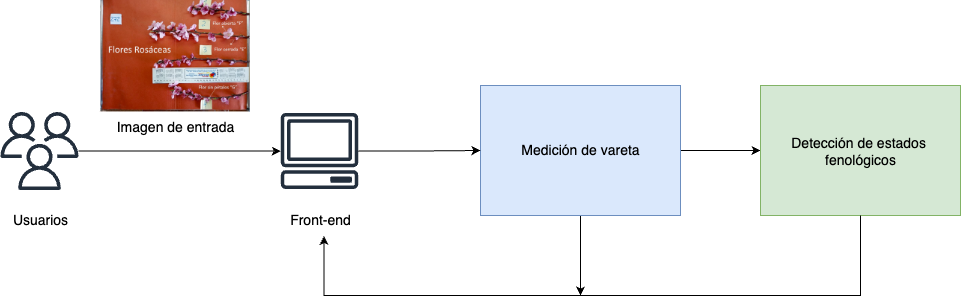
\includegraphics[scale=.35]{./Figures/arq1.drawio.png}
	\caption{Arquitectura general del sistema.}
	\label{fig:sistemaGeneral}
\end{figure}

La arquitectura del módulo que estima la longitud de la vareta se puede observar en la figura \ref{fig:varetaSize}. Este módulo toma y preprocesa la imagen de entrada, posteriormente detecta la regla que es el objeto de referencia y procede a tomar las mediciones en píxeles de dicho elemento. Luego, se hace una conversión de píxeles a centímetros. Una vez finalizada la conversión, se detectan las varetas presentes en la imagen y se calculan sus dimensiones, se revisa la orientación de la foto y se toma la longitud de cada vareta en píxeles. Finalmente, con la conversión anterior se pasa a centímetros las mediciones de las varetas, se anotan los resultados en una tabla y son enviados al siguiente módulo. Por otro lado, la imagen con las mediciones se muestra por pantalla.

Este módulo se detalla con más a profundidad en este mismo capítulo.

\begin{figure}[htpb]
	\centering
	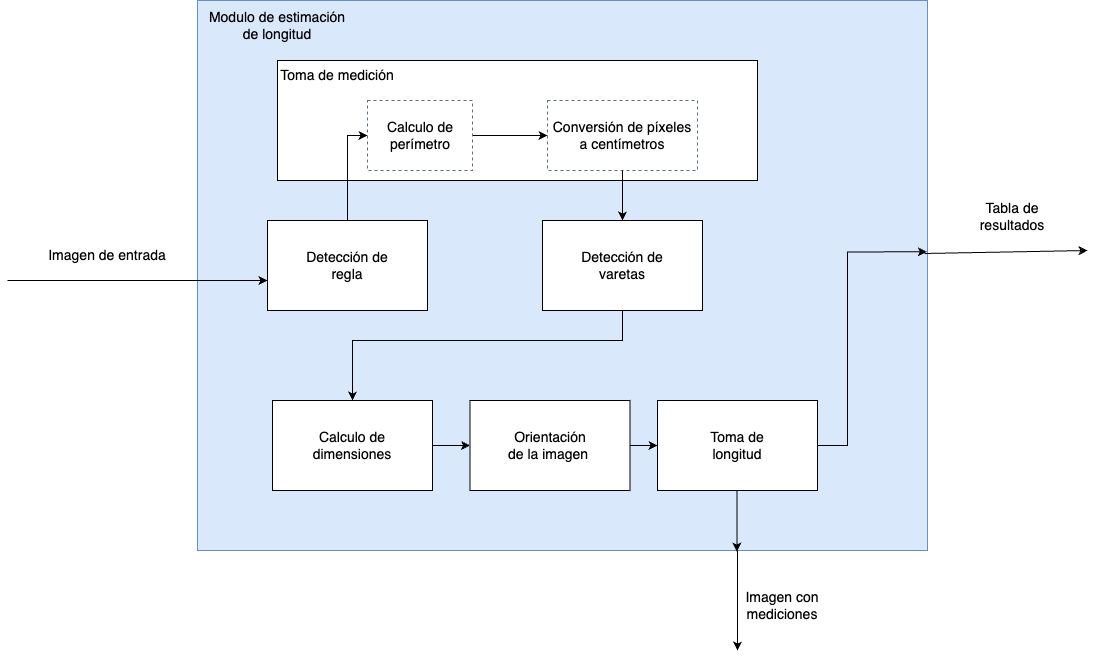
\includegraphics[scale=.35]{./Figures/medicionVareta.drawio.png}
	\caption{Módulo de estimación de longitud.}
	\label{fig:varetaSize}
\end{figure}

La arquitectura del módulo de detección y procesamiento se presenta en la figura \ref{fig:densidadDeFlores}. La entrada a este módulo es la imagen original donde se le aplica un preprocesamiento y posteriormente se pasa por un modelo que detecta los estados fenológicos de las flores de duraznero y sus varetas. Luego, se realiza un postprocesamiento de los resultados para conocer el número de flores totales que se encuentran en la imagen y un conteo de las mismas por vareta. Por último, se extraen las flores detectadas por vareta y son enviadas al clasificador para determinar su tipo.

Más adelante en este mismo capítulo se dará más información detallada de este módulo y de otros bloques del sistema que cumplen una función importante para generar los resultados deseados.

Cabe destacar que la realización de este sistema se llevó a cabo en el lenguaje de programación \textit{Python} y se encuentra diseñado para funcionar en una computadora local bajo un ambiente virtualizado. 

\begin{figure}[htp]
	\centering
	\includegraphics[scale=.3]{./Figures/DetecciónFlor.drawio.png}
	\caption{Módulo de detección y procesamiento.}
	\label{fig:densidadDeFlores}
\end{figure}
\newpage
\section{Preparación de los datos}

La preparación de los datos es una de las partes más criticas durante el desarrollo de un modelo de aprendizaje. Esto debido a que si los datos no se encuentran en las condiciones adecuadas para su uso en un modelo de IA, el modelo no tendrá un buen rendimiento. 

El presente trabajo requirió la generación de distintos etiquetados para el conjunto de datos original, debido a la cantidad de modelos utilizados durante su desarrollo.

\subsection{Análisis exploratorio}
\label{section3.2.1}
El conjunto de datos original provisto por el INTA contiene las características que se indican en la tabla \ref{tab:flores}. En general, las fotos presentan distintas dimensiones y orientaciones (vertical u horizontal). Por otro lado, se desconoce el tipo de cámara utilizada y el ángulo siempre es cenital.


\begin{table}[h]
	\centering
	\caption{Características de las fotos de duraznos.}
	\begin{tabular}{c c c l}    
		\toprule
		\textbf{Formato}     & \textbf{Cantidad} & \textbf{Resolución} & \textbf{Observaciones}\\
		\midrule
		JPG                  & 286               &  Variable &  Cuatro varetas por foto.\\		
		\bottomrule
		\hline
	\end{tabular}
	\label{tab:flores}
\end{table}
 
Las imágenes tienen un fondo naranja y en ocasiones contienen partes grises. Esto debido a que las varetas de duraznero fueron posadas sobre una cartulina color naranja y a veces por las dimensiones de las varetas, se toma parte de la mesa de color gris.

Por otro lado, las fotos presentan cambios de brillo e iluminación, generando distintas tonalidades de los colores de fondo y de las flores. 

Los elementos que se observan generalmente en las fotos provistas por el cliente incluyen: una regla, cuatro varetas, una cartulina de fondo, cuatro etiquetas que identifican las varetas y en ocasiones objetos que no forman parte de la detección o que no aportan información.

En la figura \ref{fig:three graphs}, se puede observar algunos ejemplos de fotos con las características que se describieron anteriormente.

\begin{figure}[ht]
     \centering
     \begin{subfigure}[b]{0.4\textwidth}
         \centering
         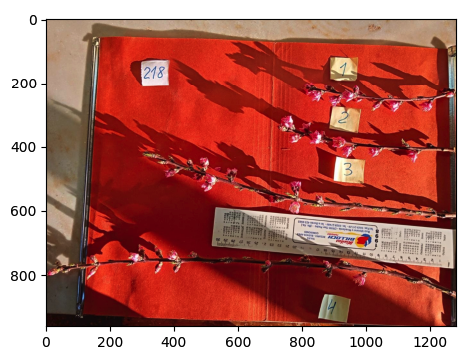
\includegraphics[scale=.4]{./Figures/flor_muestra5.png}
         \caption{Foto de muestra 1.}
         \label{fig:1de3}
     \end{subfigure}
     \hfill
     \begin{subfigure}[b]{0.4\textwidth}
         \centering
         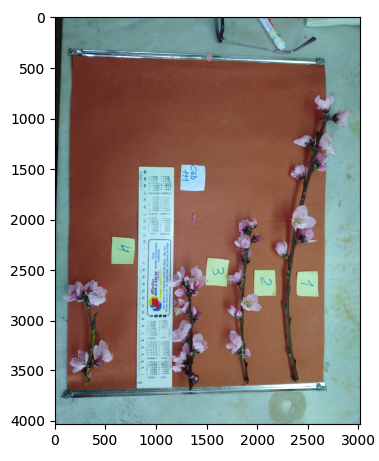
\includegraphics[scale=.4]{./Figures/flor_muestra3.png}
         \caption{Foto de muestra 2.}
         \label{fig:2de3}
     \end{subfigure}
     \hfill
     \begin{subfigure}[b]{0.5\textwidth}
         \centering
         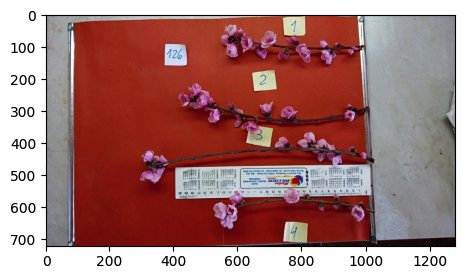
\includegraphics[scale=.45]{./Figures/flor_muestra6.png}
         \caption{Foto de muestra 3.}
         \label{fig:3de3}
     \end{subfigure}
        \caption{Fotos de muestra del conjunto de datos.}
        \label{fig:three graphs}
\end{figure}

Es importante mencionar que, las fotos de varetas tomadas por el cliente, están clasificadas por el tipo de flor que poseen las varetas. Es decir, una foto solo va a contener varetas con flores del tipo rosáceas o campanuláceas, pero no ambos tipos de flor en una misma imagen. En la figura \ref{fig:two graphs} se muestran dos fotos de varetas, una que contiene flores rosáceas y otra que contiene flores campanuláceas.

\begin{figure}[ht]
     \centering
     \begin{subfigure}[b]{0.3\textwidth}
         \centering
         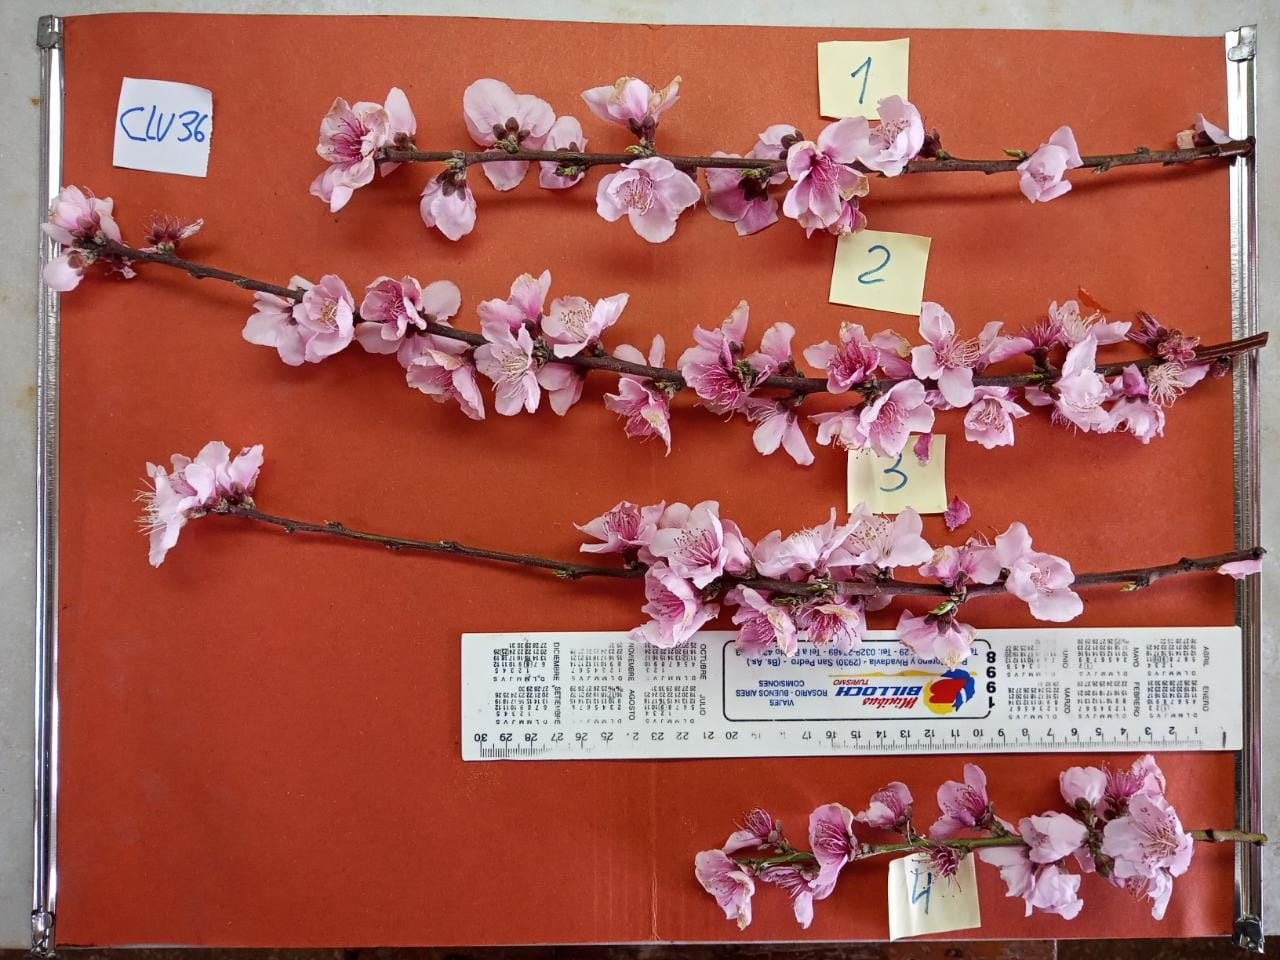
\includegraphics[scale=.13]{./Figures/flor_rosacea.jpg}
         \caption{Foto de varetas con flores rosáceas.}
         \label{fig:1de23}
     \end{subfigure}
     \hfill
     \begin{subfigure}[b]{0.45\textwidth}
         \centering
         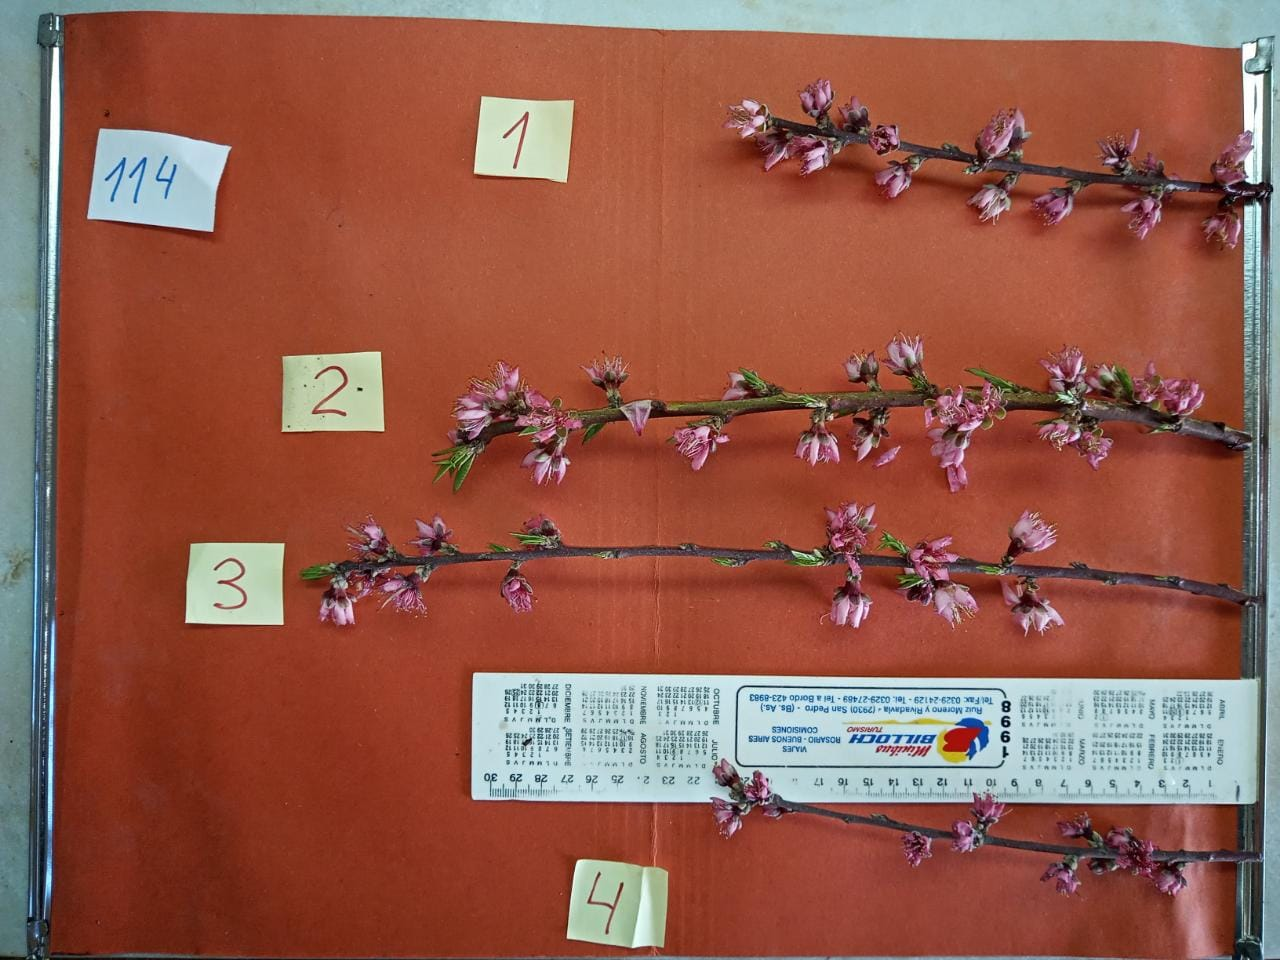
\includegraphics[scale=.13]{./Figures/flor_camp.jpg}
         \caption{Foto de varetas con flores campanuláceas.}
         \label{fig:2de23}
     \end{subfigure}
        \caption{Fotos de varetas de duraznero con su tipo flor.}
        \label{fig:two graphs}
\end{figure}

\newpage

Cabe destacar que en una foto de varetas de duraznero, se encuentran varias flores y cada flor posee un estado fenológico. Los estados fenológicos que se pueden encontrar son: flor abierta, flor cerrada y flor sin pétalos respectivamente. En la figura \ref{fig:estadoFeno} se observan dichos estados fenológicos para la flor de duraznero del tipo rosácea.

\begin{figure}[!htp]
     \centering
     \begin{subfigure}[b]{0.4\textwidth}
         \centering
         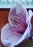
\includegraphics[scale=2]{./Figures/4 (2)_cropped0.jpg}
         \caption{Flor abierta.}
         \label{fig:1de33}
     \end{subfigure}
     \hfill
     \begin{subfigure}[b]{0.2\textwidth}
         \centering
         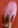
\includegraphics[scale=2]{./Figures/33 (2)_cropped45.jpg}
         \caption{Flor cerrada.}
         \label{fig:2de33}
     \end{subfigure}
     \hfill
     \begin{subfigure}[b]{0.3\textwidth}
         \centering
         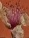
\includegraphics[scale=2]{./Figures/39_cropped12.jpg}
         \caption{Flor sin pétalos.}
         \label{fig:3de33}
     \end{subfigure}
        \caption{Fotos de estados fenológicos de la flor de duraznero.}
        \label{fig:estadoFeno}
\end{figure}

\subsubsection{Balanceo del conjunto de datos antes del etiquetado}

El conjunto de datos cuenta con un total de 286 imágenes en total, donde, 57 imágenes contienen varetas con flores del tipo campanuláceas, y 229 contienen varetas con flores del tipo rosáceas. Por lo tanto, se considera que el conjunto de datos se encuentra desbalanceado con respecto al tipo de flor. 

\subsection{Etiquetado del conjunto de datos}

El conjunto de datos dado por el cliente fue etiquetado utilizando una herramienta llamada \textit{Roboflow}. El etiquetado con \textit{Roboflow} es simple y se puede utilizar para múltiples tareas relacionadas a visión por computadora. Por otro lado, el presente trabajo requirió varios etiquetados del mismo conjunto de datos, debido a, los distintos modelos que se entrenaron para su realización.

Todos los modelos utilizados exceptuando el clasificador, utilizaron un etiquetado del tipo de detección de objetos, donde se delimitan los objetos de interés con \textit{bounding boxes}. El etiquetado por modelo se detalla en la siguiente lista:

\begin{enumerate}
	\item Detección de estados fenológicos: las etiquetas para el entrenamiento de este modelo fueron cinco y representan cada estado fenológico de la flor de duraznero. Estas etiquetas son: flor abierta, flor cerrada, flor sin pétalos, incierto y vareta. El tipo de etiquetado fue de detección de objetos.
	\item Detección de regla: para este etiquetado se utilizó el mismo \textit{dataset}, pero solo se tomó en cuenta la regla, por lo tanto, solo cuenta con esta única etiqueta y el tipo de etiquetado es de detección de objetos.
	\item Detección de vareta: solo se etiquetaron las varetas, el motivo del porque se vuelve a hacer un etiquetado para este objeto se explica en secciones más adelante.
\end{enumerate}

El conjunto de datos utilizado para entrenar el clasificador de flores se generó y etiquetó mediante un algoritmo, que emplea el modelo que detecta los estados fenológicos, y posteriormente recorta cada flor detectada. Luego para distinguir entre las flores rosáceas y campanuláceas, se procesaron imágenes de ejemplares de cada tipo por separado, almacenando los resultados en archivos distintos clasificados por categoría.

Finalmente, por motivos de tiempo no se lograron etiquetar las 286 imágenes para cada caso. Los detalles de la cantidad de imágenes etiquetadas por conjunto de datos se encuentra en la tabla \ref{tab:etiquetado}. 

\begin{table}[h]
	\centering
	\caption{Cantidad de fotos etiquetadas por modelo.}
	\begin{tabular}{l c }    
		\toprule
		\textbf{Modelo}     & \textbf{Cantidad de imágenes etiquetadas} \\
		\midrule
		Detector de estados fenológicos.                  & 140 \\
		Detector de regla.                  & 131 \\
		Detector de vareta.                  & 101 \\		
		\bottomrule
		\hline
	\end{tabular}
	\label{tab:etiquetado}
\end{table}

\subsubsection{Balanceo del conjunto de datos después del etiquetado}
\label{desbalanceAfterLabeled}

El conjunto de datos para el detector de los estados fenológicos de la flor tenía un desbalance que se puede observar en la figura \ref{fig:desbalanceoDeteccion}. La clase mayoritaria vendría siendo flor abierta que es el estado fenológico con más presencia en las 140 fotos etiquetadas. Las consecuencias y la solución a este problema de desbalanceo para el detector de estados fenológicos se explica más delante en la presente memoria.

\begin{figure}[ht]
	\centering
	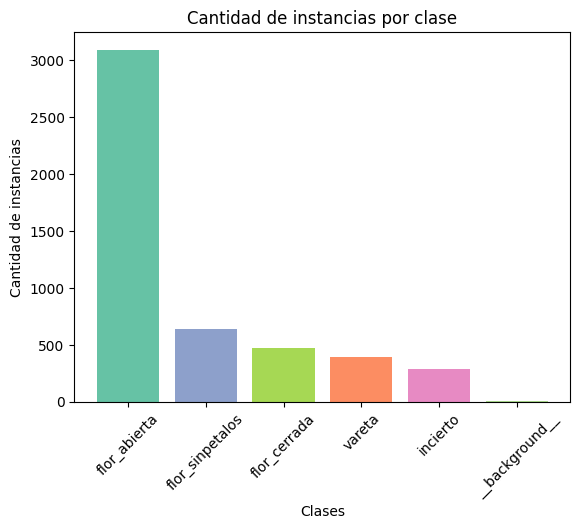
\includegraphics[scale=.65]{./Figures/desbalanceo_detector.png}
	\caption{Desbalanceo de clases para el detector de estados fenológicos de la flor de duraznero.}
	\label{fig:desbalanceoDeteccion}
\end{figure}
\newpage

Por otro lado, el conjunto de datos para el clasificador de flores contaba con un desbalance, entre la cantidad de flores rosáceas y campanuláceas. Este desbalance se observa en la figura \ref{fig:desbalanceoClass}.

\begin{figure}[ht]
	\centering
	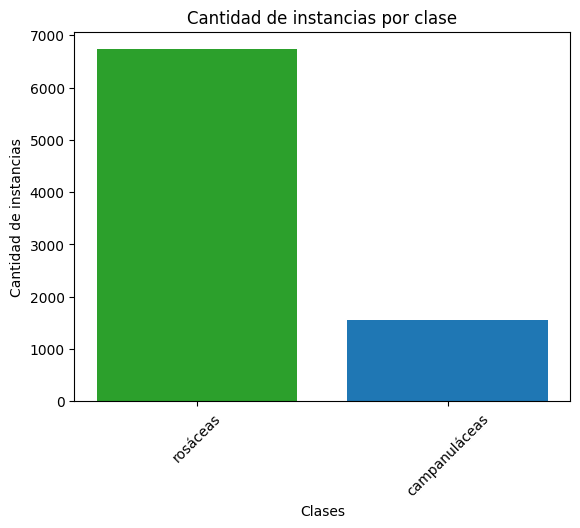
\includegraphics[scale=.53]{./Figures/tipodeflor_desbalance.png}
	\caption{Desbalanceo de clases para el clasificador de flores de duraznero.}
	\label{fig:desbalanceoClass}
\end{figure}
\newpage
\subsection{Aumento de los datos}
\label{aumentoDatos}
Se utilizó \textit{data augmentation} para incrementar la cantidad de imágenes para el conjunto de datos destinados al modelo de detección de los estados fenológicos, además las transformaciones de imágenes aplicadas buscan que el modelo sea capaz de generalizar mejor a pesar de encontrar cambios de brillo, iluminación, rotaciones, etc. Por otro lado, también se hizo uso de esta técnica para intentar balancear el conjunto de datos destinado al clasificador de flores.

Para el detector de estados fenológico de las flores de duraznero se implementaron las siguientes transformaciones:

\begin{enumerate}
	\item 90 grados de rotación en sentido horario y anti horario.
	\item Cambio de brillo entre un -25\% y 25\%. 
	\item Desenfoque un 1 px.
	\item Cambio de brillo por \textit{bounding box}.
\end{enumerate}

El total de imágenes aumento a 336. Sin embargo, es de tener en cuenta que el número de imágenes disponible sigue siendo inferior al recomendado para el entrenamiento y validación de los distintos modelos de aprendizaje utilizados en la presente memoria. Por otro lado, con esta técnica no se pudo resolver el desbalance de datos observado en la figura \ref{fig:desbalanceoClass}, debido a que no hay una transformación directa de la imagen que permita la eliminación de las clases mayoritarias presentes en la detección, más adelante en la presente memoria se explica el método implementado para mitigar el desbalanceo en este caso.

El detector de vareta también contó con un aumento de los datos para mejorar el rendimiento del modelo de detección utilizado y para incrementar la cantidad de muestras que se tenían a un total de 243 imágenes. Las transformaciones utilizadas fueron:

\begin{enumerate}
	\item Rotación horizontal.
	\item Cambio de brillo entre un -15\% y 15\%. 
	\item Desenfoque un 1 px.
	\item Ruido hasta un 0.1\% en píxeles.
\end{enumerate}

Para el clasificador de flores se aplicaron transformaciones que involucraban giros o rotaciones aleatorias de 0 a 180 grados. Esto se hizo tres veces para incrementar el número de flores campanuláceas e igualar la cantidad de muestras de las flores rosáceas.

\section{Módulo de estimación de longitud}

El objetivo de este módulo es estimar la longitud de las varetas de duraznero presentes en la imagen. Para esto, se utilizó el enfoque de encontrar un objeto de referencia al que se le conocen sus dimensiones en centímetros y, en base a estas dimensiones, se calculan las del objeto objetivo que en este caso serían las varetas. 

En las fotos provistas por el INTA, como se menciona en la sección \ref{section3.2.1}, contienen una regla de 30 centímetros de largo y 5 de ancho. Esta regla se utilizó como objeto de referencia para la estimación de longitud de las varetas. Para su detección, se tuvo que aplicar \textit{transfer learning} y \textit{fine tunning} a un modelo de detección. El modelo base utilizado fue \textit{YOLOv8n} de Ultralytics que fue preentrenado con el conjunto de datos de COCO.

Una vez detectada la regla, se toman las dimensiones del \textit{bounding box} y se calcula su perímetro en píxeles. Luego, sabiendo que el perímetro en centímetros es 70, se hace una división del perímetro en píxeles entre el perímetro en centímetros, lo que termina dando como resultado, la razón matemática que representa la cantidad de píxeles en la imagen que representan 1 centímetro. Con esto, se obtuvo la conversión para poder aplicarla a los demás objetos en la imagen.

Posteriormente, se realiza la detección de las varetas y para esto, se entrenó un modelo \textit{YOLOv8n} de Ultralytics preentrenado que en este caso al igual que para el detector de regla, el \textit{bounding box} proporcionado durante el etiquetado, es lo más preciso con el contorno real del objeto, debido a que las dimensiones de este delimitador son fundamentales para la estimación de longitud que se desea obtener. 

Cuando se detectan las varetas, se hace la conversión de píxeles a centímetros tomando los anchos y altos de los \textit{bounding boxes} y dividiendolos entre la razón matemática obtenida anteriormente. El resultado obtenido es la estimación en centímetros del alto y ancho de los \textit{bounding boxes}. Con este dato, se toman en cuenta dos cosas. Si el ancho es más grande que el alto en los \textit{bounding boxes}, entonces, la imagen tiene una orientación horizontal. Por lo tanto, el ancho en este caso es la estimación de longitud tanto para la regla como para las varetas. En caso contrario, la imagen se encuentra en orientación vertical y el alto es efectivamente la estimación de longitud de los objetos.

Por otro lado, cabe destacar que las detecciones de las varetas se organizan de menor a mayor recorriendo la imagen en el eje X (izquierda a derecha), si la imagen es vertical. En el caso contrario, se hace de la misma forma, pero sobre el eje Y. Con esta técnica es posible identificar las varetas que se detectan y su respectiva estimación de longitud.

Por último, se imprime por pantalla la imagen con las detecciones y las mediciones, además se muestra una tabla con los resultados obtenidos en este módulo. Esta tabla posteriormente se une con el resultado del módulo de detección y procesamiento. En la figura \ref{fig:modulo1} se observa un ejemplo del resultado obtenido por pantalla.

%\begin{figure}[ht]
%	\centering
%	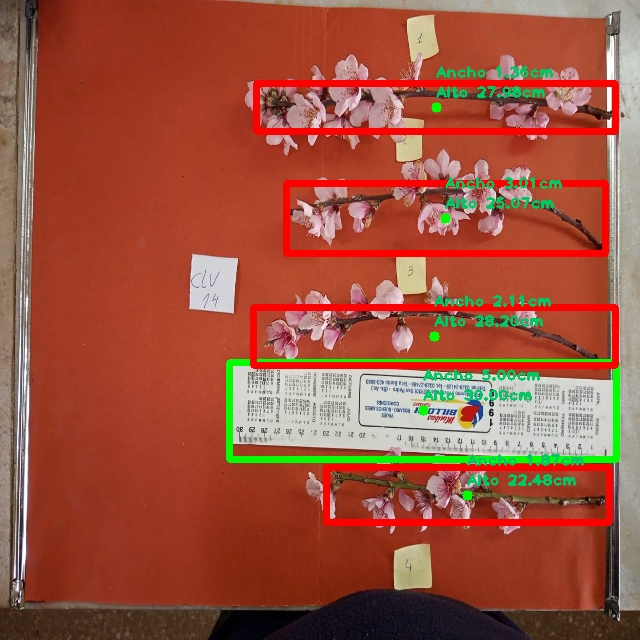
\includegraphics[scale=.4]{./Figures/vareta_size.jpeg}
%	\caption{Desbalanceo de clases para el clasificador de flores de duraznero.}
%	\label{fig:desbalanceoClass}
%\end{figure}

\begin{figure}[ht]
     \centering
     \begin{subfigure}[b]{0.3\textwidth}
         \centering
         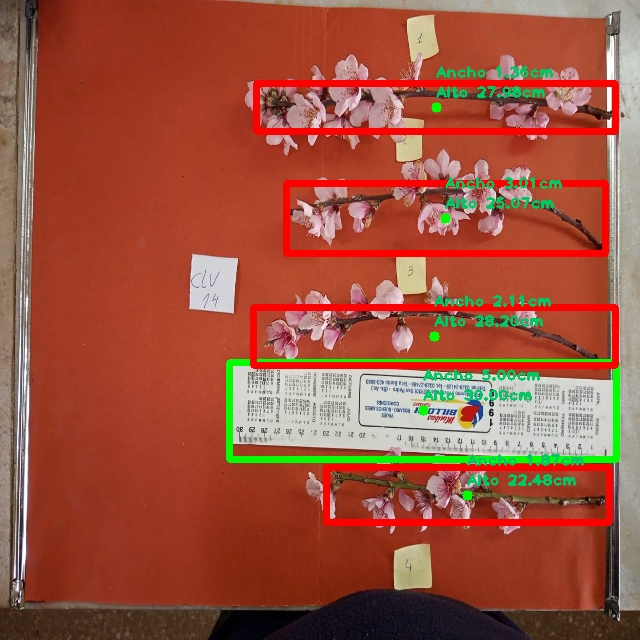
\includegraphics[scale=0.4]{./Figures/vareta_size.jpeg}
         \caption{imagen con estimaciones de dimensiones.}
         \label{fig:1de33}
     \end{subfigure}
     \hfill
     \begin{subfigure}[b]{0.3\textwidth}
         \centering
         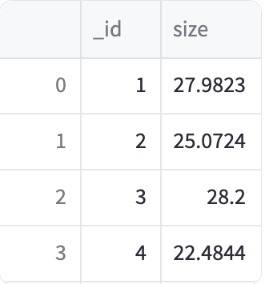
\includegraphics[scale=.4]{./Figures/vareta_size_table.jpg}
         \caption{Tabla con estimaciones de dimensiones.}
         \label{fig:2de33}
     \end{subfigure}
        \caption{Resultados del módulo de estimación de longitud.}
        \label{fig:modulo1}
\end{figure}
\newpage

\section{Módulo de detección y procesamiento}

El propósito de este módulo es detectar los estados fenológicos de la flores de duraznero, hacer un conteo total de la cantidad de flores presentes y por vareta, y por último clasificar si las flores por vareta son campanuláceas o rosáceas.

\subsection{Detección de estados fenológicos}

Para la detección de los estados fenológicos se utilizó el modelo de detección \textit{YOLOv8n} de Ultralytics, preentrenado con el conjunto de datos de COCO. Se le aplicó \textit{fine tunning} para ajustarlo a este caso de uso y como parte de la búsqueda del mejor modelo para realizar dicha detección, se probó contra \textit{Faster R-CNN} que es un detector de dos etapas. Al final de las pruebas se seleccionó el modelo con mejores métricas de \textit{mAP}, que en este caso fue \textit{YOLOv8n}. En el siguiente capítulo se detallarán dichas pruebas.

Los resultados de esta detección no solo incluyen la localización e identificación de cada estado fenológico de cada flor, sino también la detección de la vareta. El motivo para detectar nuevamente la vareta va relacionado a la toma de regiones de interés que serán de utilidad más adelante en este mismo módulo.  

En la figura \ref{fig:deteccionEjem}, se pueden observar los resultados que se obtienen del detector de estados fenológicos de la flor de duraznero.

\begin{figure}[ht]
	\centering
	\includegraphics[scale=.35]{./Figures/detección.jpeg}
	\caption{Imagen de salida del detector de estados fenológicos.}
	\label{fig:deteccionEjem}
\end{figure}

\subsection{Conteo de flores}

Para realizar el conteo total de flores por imagen, primero se posprocesan las detecciones obtenidas del detector de estados fenológicos. Luego, se buscan las centroides de cada \textit{bounding box} y se filtran las detecciones pertenecientes a algunas de las siguientes clases: flor abierta, flor cerrada, flor sin petalos e incierto. Posteriormente, a través de un script, se crea una lista de flores detectadas y se utilizan las centroides tomadas anteriormente para evitar la toma de detecciones que tuvieran una misma posición. De esta  forma, no se toman en cuenta las detecciones duplicadas.

Para realizar el conteo de flores por vareta, se requirió de otro posprocesamiento de los resultados obtenidos del detector de estados fenológicos. En este caso, se toma en cuenta las detecciones pertenecientes a la clase vareta y, al igual que el módulo que estima la longitud de las varetas, se busca el ancho y el alto de los \textit{bounding boxes} de esta clase para, posteriormente, identificar si la imagen posee una orientación horizontal o en vertical. El dato de la orientación de la imagen es importante para conocer como se tiene que recorrer la foto, de forma que se mantenga el mismo identificador de vareta que se utiliza en el módulo de estimación de longitudes.

Una vez se conoce la orientación de la imagen, se ordenan las detecciones de las varetas y se empieza a recorrer la foto en el eje X si es vertical o en el eje Y si es horizontal. En cada iteración se crea un identificador para cada vareta encontrada. Durante estás iteraciones, para aislar cada vareta de forma de poder contar sus flores, se tuvo que utilizar el enfoque de buscar y crear regiones de interés.

La región de interés se genera a partir de las coordenadas del \textit{bounding box} perteneciente a la clase vareta. Una vez se obtienen dichas coordenadas, se oscurece la imagen pasando cada píxel a cero y se encienden los píxeles dentro de la región de interés. Posteriormente, se realiza una operación \textit{bitwise and} entre la imagen con la región de interés y la original, dando como resultado, la imagen oscurecida con solo una vareta iluminada. Este procedimiento lo realiza el script por cada vareta encontrada y en el orden mencionado anteriormente.

Adicionalmente, por cada región de interés, se procede a filtrar las centroides pertenecientes a dicha región. De esta forma, se genera una lista con las flores encontradas que representa la cantidad de flores por vareta. En la figura \ref{fig:regionInte}, se puede observar un ejemplo del resultado de esta operación. 

\begin{figure}[ht]
     \centering
     \begin{subfigure}[b]{0.4\textwidth}
         \centering
         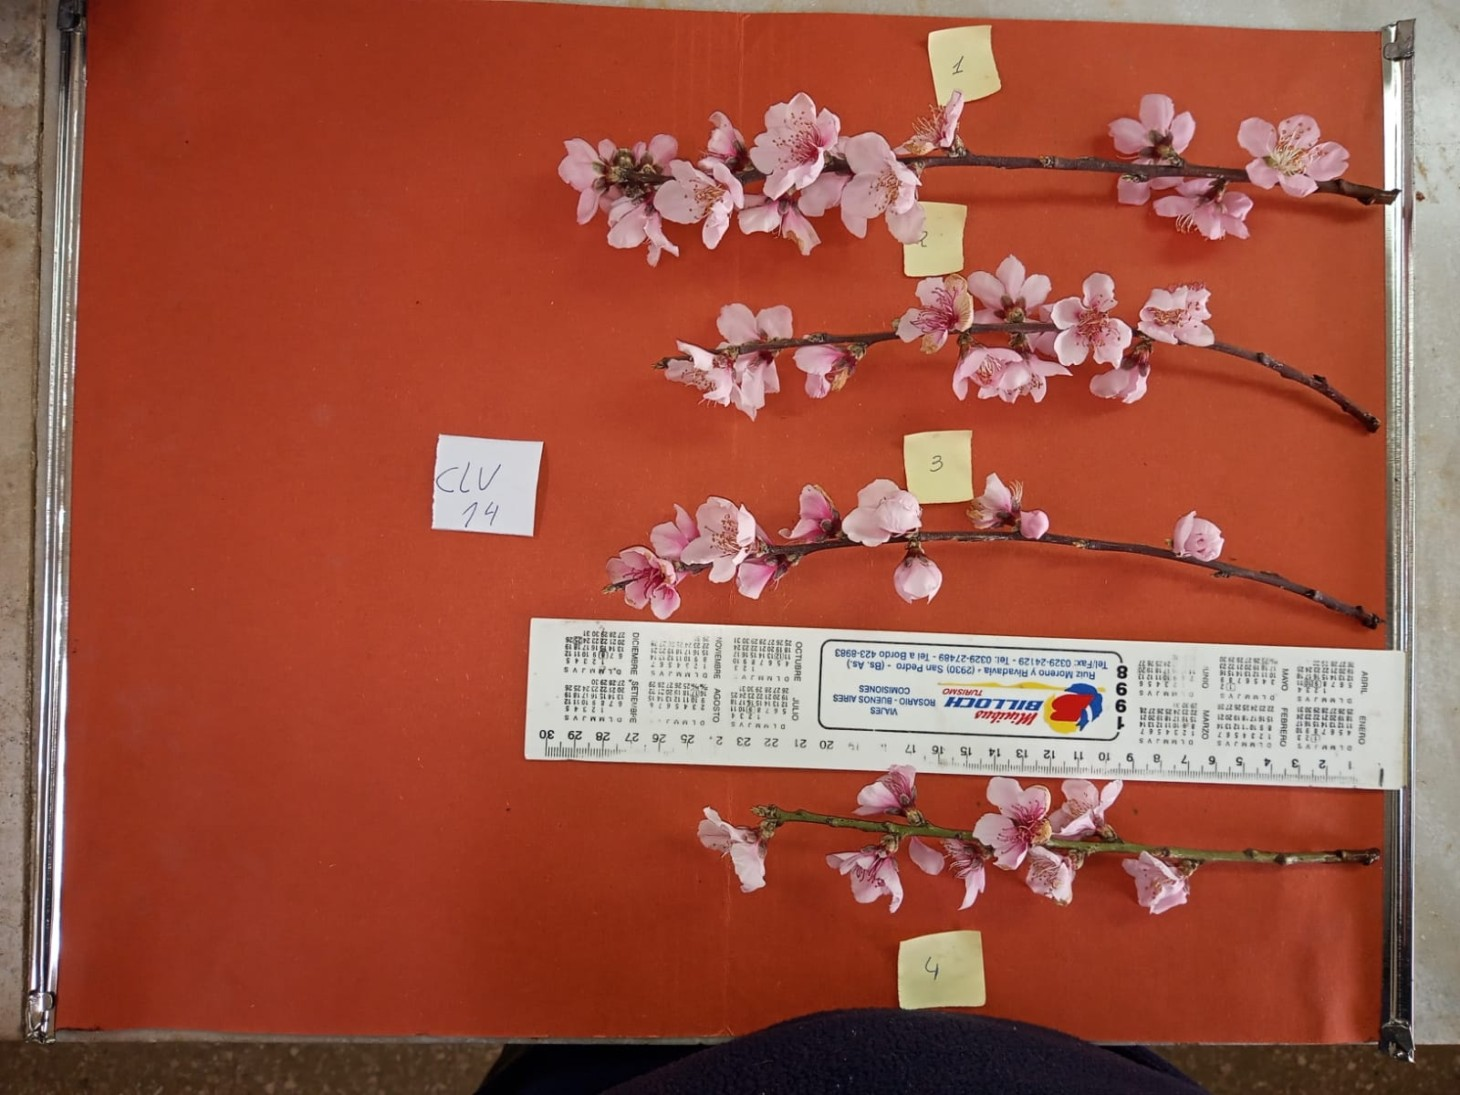
\includegraphics[scale=0.13]{./Figures/original.jpeg}
         \caption{imagen original.}
         \label{fig:1de34}
     \end{subfigure}
     \hfill
     \begin{subfigure}[b]{0.4\textwidth}
         \centering
         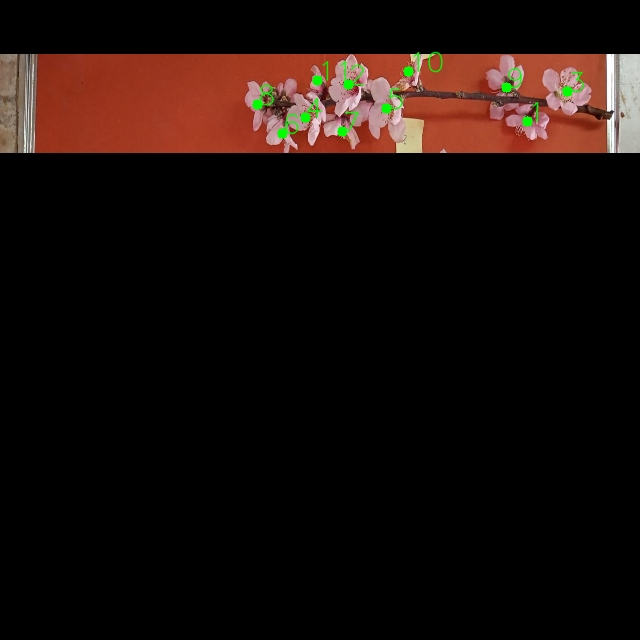
\includegraphics[scale=0.25]{./Figures/1stCount.jpeg}
         \caption{Primera región de interés.}
         \label{fig:2de34}
     \end{subfigure}
        \caption{Ejemplo de conteo de flores por vareta con regiones de interés.}
        \label{fig:regionInte}
\end{figure}

Cabe destacar que para que este procedimiento sea efectivo, es necesario que cada vareta tenga una distancia apropiada entre si. Bajo esta condición, se evita tomar las flores pertenecientes a una vareta vecina. 

\subsection{Clasificador de flores}

El clasificador de flores de duraznero es la última fase que recorre el sistema antes de finalizar el proceso y generar la tabla final de resultados. El desarrollo de este componente requirió diseñar una red neuronal convolucional para hacer distinción entre flores del tipo rosáceas o campanuláceas. En este caso, no se realizó \textit{transfer learning} dado que la clasificación no era muy compleja y se tenía una gran cantidad de muestras para el entrenamiento. En la tabla \ref{tab:FlowerCNN}, se puede observar la arquitectura de esta red neuronal convolucional.

\begin{table}[h]
	\centering
	\caption{Arquitectura de CNN para clasifiación de flores de duraznero.}
	\begin{tabular}{l c c}    
		\toprule
		\textbf{Capaz}     & \textbf{Dimensiones de salida} & \textbf{Parámetros} \\
		\midrule
		Conv2d-1.          & [-1, 16, 25, 25] &  448\\
		MaxPool2d-2.       & [-1, 16, 12, 12] & 0\\
		Conv2d-3.          & [-1, 32, 12, 12] & 4,640 \\
		MaxPool2d-4.       & [-1, 32, 6, 6]   & 0 \\
		Conv2d-5.          & [-1, 64, 6, 6]   & 18,496 \\
		MaxPool2d-6.       & [-1, 64, 3, 3]   & 0 \\	
		Linear-7.          & [-1, 128]        & 73,856 \\
		Dropout-8.         & [-1, 128]        & 0 \\
		Linear-9.          & [-1, 2]          & 258 \\	
		\bottomrule
		\hline
	\end{tabular}
	\label{tab:FlowerCNN}
\end{table}  
\newpage
Esta red convolucional cuenta con un total de 97.698 parámetros entrenables. Por otro lado, se le tuvo que aplicar métodos como regulación \textit{L2} y \textit{DropOut} para disminuir el sobre ajuste. Las pruebas del rendimiento de este modelo y el sobre ajuste se explicarán con más detalle en el capítulo siguiente.

Este modelo se integra y se ejecuta luego de encontrar y delimitar la región de interés en cada vareta. Al momento de tomar la región de interés y contar la cantidad de flores en dicha región, se filtra por aquellas detecciones que representan a las clases flor abierta y flor cerrada, para posteriormente recortar dicha detección utilizando sus coordenadas provistas por el \textit{bounding box}. Una vez recortada la imagen de la flor, se redimensiona a una resolución de 25 x 25 y se envía al clasificador. Finalmente, el clasificador a través de su última capa totalmente conectada, produce una probabilidad para cada clase, donde se selecciona la clase con la probabilidad más alta. Este proceso se repite por cada flor abierta y cerrada encontrada en la vareta. 

Al final, cuando se clasificaron todas las flores abiertas y cerradas de una misma vareta, se guarda el resultado en un arreglo de datos y se toma la categoría con mayor aparición en dicho arreglo. Es decir, este arreglo permite que si el clasificador se equivoca categorizando una flor, se pueda emendar dicho error con un proceso de votación. Este paso es importante porque una misma vareta no puede tener más de una clase. 

Por otro lado, este proceso iterativo de recorrer la imagen y clasificar cada vareta con un tipo de flor, permite que en el futuro, se pueda tener una imagen que contenga varetas con distintas categorías.
\newpage
\section{Integración de módulos y generación de resultado}

La integración de los módulos se realizó a través del lenguaje de programación \textit{Python}, donde ambos componentes se ejecutan desde el script principal y de forma secuencial. De esta forma, como se mostró en la figura \ref{fig:sistemaGeneral}, el primer módulo en recibir la imagen es el de estimación de longitud y posteriormente se ejecuta el de detección y procesamiento.

En cada módulo se genera un diccionario de \textit{Python}, que contiene el resultado de dicha operación, ambos resultados contienen una variable en común. Esta variable es la identificación de cada vareta que se produce durante el recorrido que realiza cada algoritmo sobre la imagen. Por este motivo, es importante que ambos algoritmos recorran la imagen de la misma forma para que esta variable sea consistente en ambos resultados.

En un paso posterior, ambos resultados de cada algoritmo se transforma a un formato de \textit{Dataframe} de \textit{Pandas} para luego concatenarlos y presentar al usuario final una única tabla de resultados.

En la figura \ref{fig:TablaResultados1} y la figura \ref{fig:TablaResultados2}, se observa un ejemplo de la tabla resultante de cada algoritmo presentada por pantalla.

\begin{figure}[ht]
	\centering
	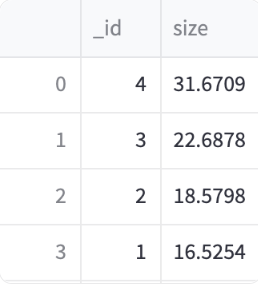
\includegraphics[scale= 0.3]{./Figures/Tabla1.png}
	\caption{Ejemplo de tabla resultante del módulo de estimación de longitud.}
	\label{fig:TablaResultados1}
\end{figure}

\begin{figure}[ht]
	\centering
	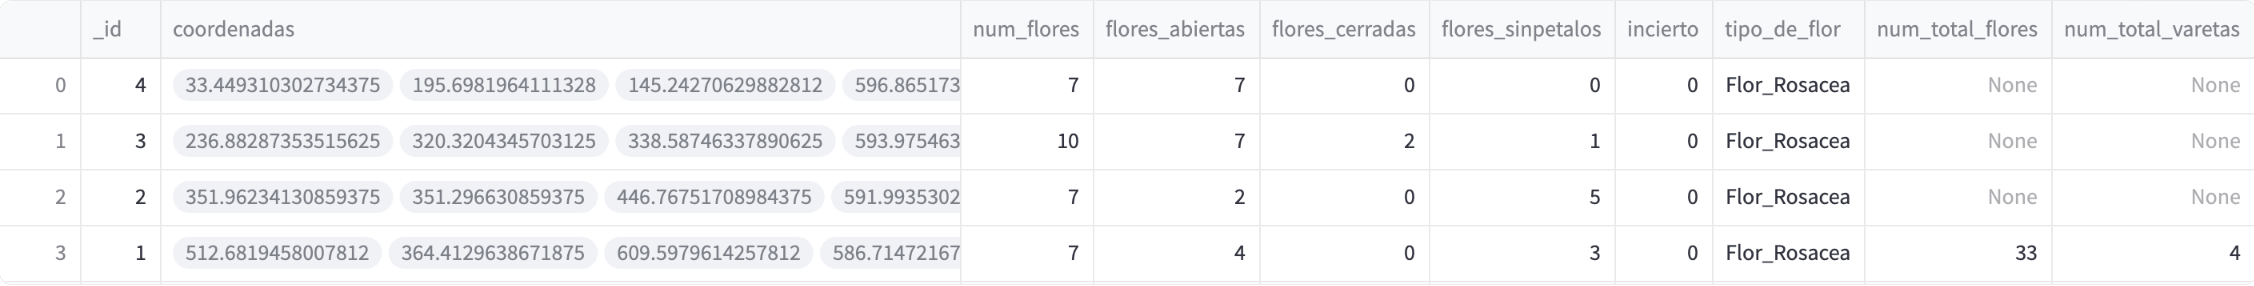
\includegraphics[width= 12cm, height= 2.5cm]{./Figures/Tabla2.png}
	\caption{Ejemplo de tabla resultante del módulo de clasificación y procesamiento.}
	\label{fig:TablaResultados2}
\end{figure}

Cabe destacar que se generaron dos botones para obtener la tabla de resultados en dos formatos distintos. El primero genera el resultado en formato CSV y el segundo produce el resultado en formato XLSX para su correcta visualización en \textit{Excel}. 

En la figura \ref{fig:TablaResultados3}, se muestra un ejemplo de ambas tablas unificadas que representan el resultado final del sistema.

\begin{figure}[ht]
	\centering
	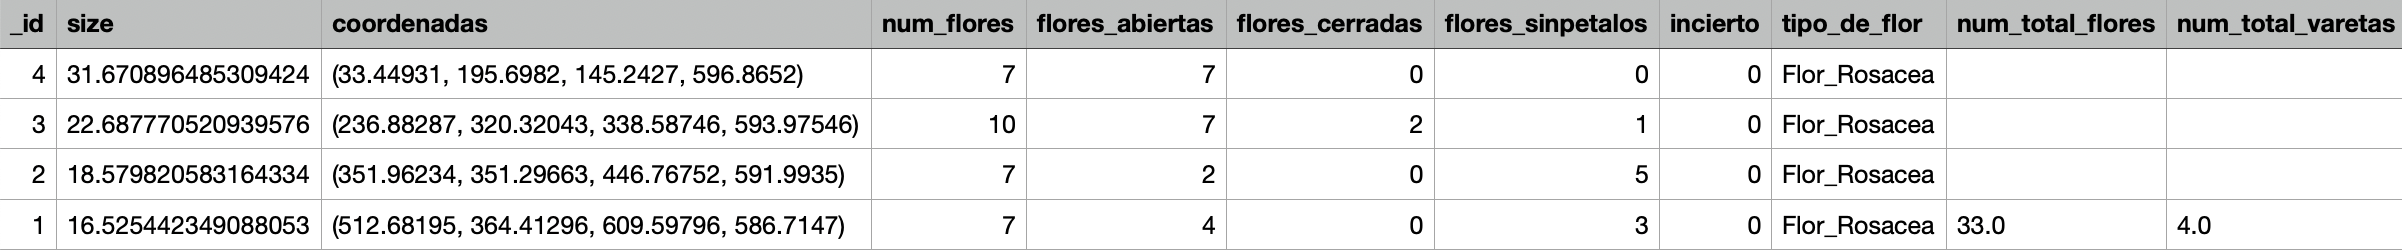
\includegraphics[width= 14cm, height= 2cm]{./Figures/Tabla3.png}
	\caption{Ejemplo de tabla unificada.}
	\label{fig:TablaResultados3}
\end{figure}

\newpage
\section{Interfaz de usuario}

La interfaz gráfica del programa fue realizada con \textit{Streamlit}, que es una herramienta que permite compartir aplicaciones \textit{web}, utilizando \textit{Python}. Adicionalmente, Esta herramienta no requiere ningún conocimiento previo en desarrollo de \textit{front end}. 

Para el desarrollo del \textit{front end} con \textit{Streamlit} y para ejecutar el proyecto en un entorno local, fue necesario crear una estructura de directorios que contuviesen los modelos de IA, los \textit{scripts} de \textit{Python} para ejecutar cada módulo, los \textit{logs} generados por el sistema y por último, para tener un conocimiento de los experimentos realizados, un directorio para guardar las \textit{notebooks} utilizadas. Para su ejecución, se creó un entorno virtual con \textit{Python}, que contiene todas las bibliotecas y dependencias necesarias.

Los \textit{scripts} de \textit{Python} son cuatro en total, donde dos ellos llamados \textit{densidad vareta.py} y \textit{vareta size.py} representan los módulos de detección y procesamiento, y estimación de longitud respectivamente. El \textit{script} de \textit{flower classifier.py} contiene la red neuronal convolucional desarrollada para el clasificador de flores. Por último, se tiene el \textit{script} principal que ejecuta la interfaz de usuario con \textit{Streamlit} y orquesta los módulos del sistema.

La interfaz de usuario cuenta con una página de presentación, donde se observa el titulo del proyecto, las tecnologías utilizadas y el propósito del mismo. En la figura \ref{fig:pantallaInicio}, se muestra un ejemplo de esta pantalla de inicio.

\begin{figure}[ht]
	\centering
	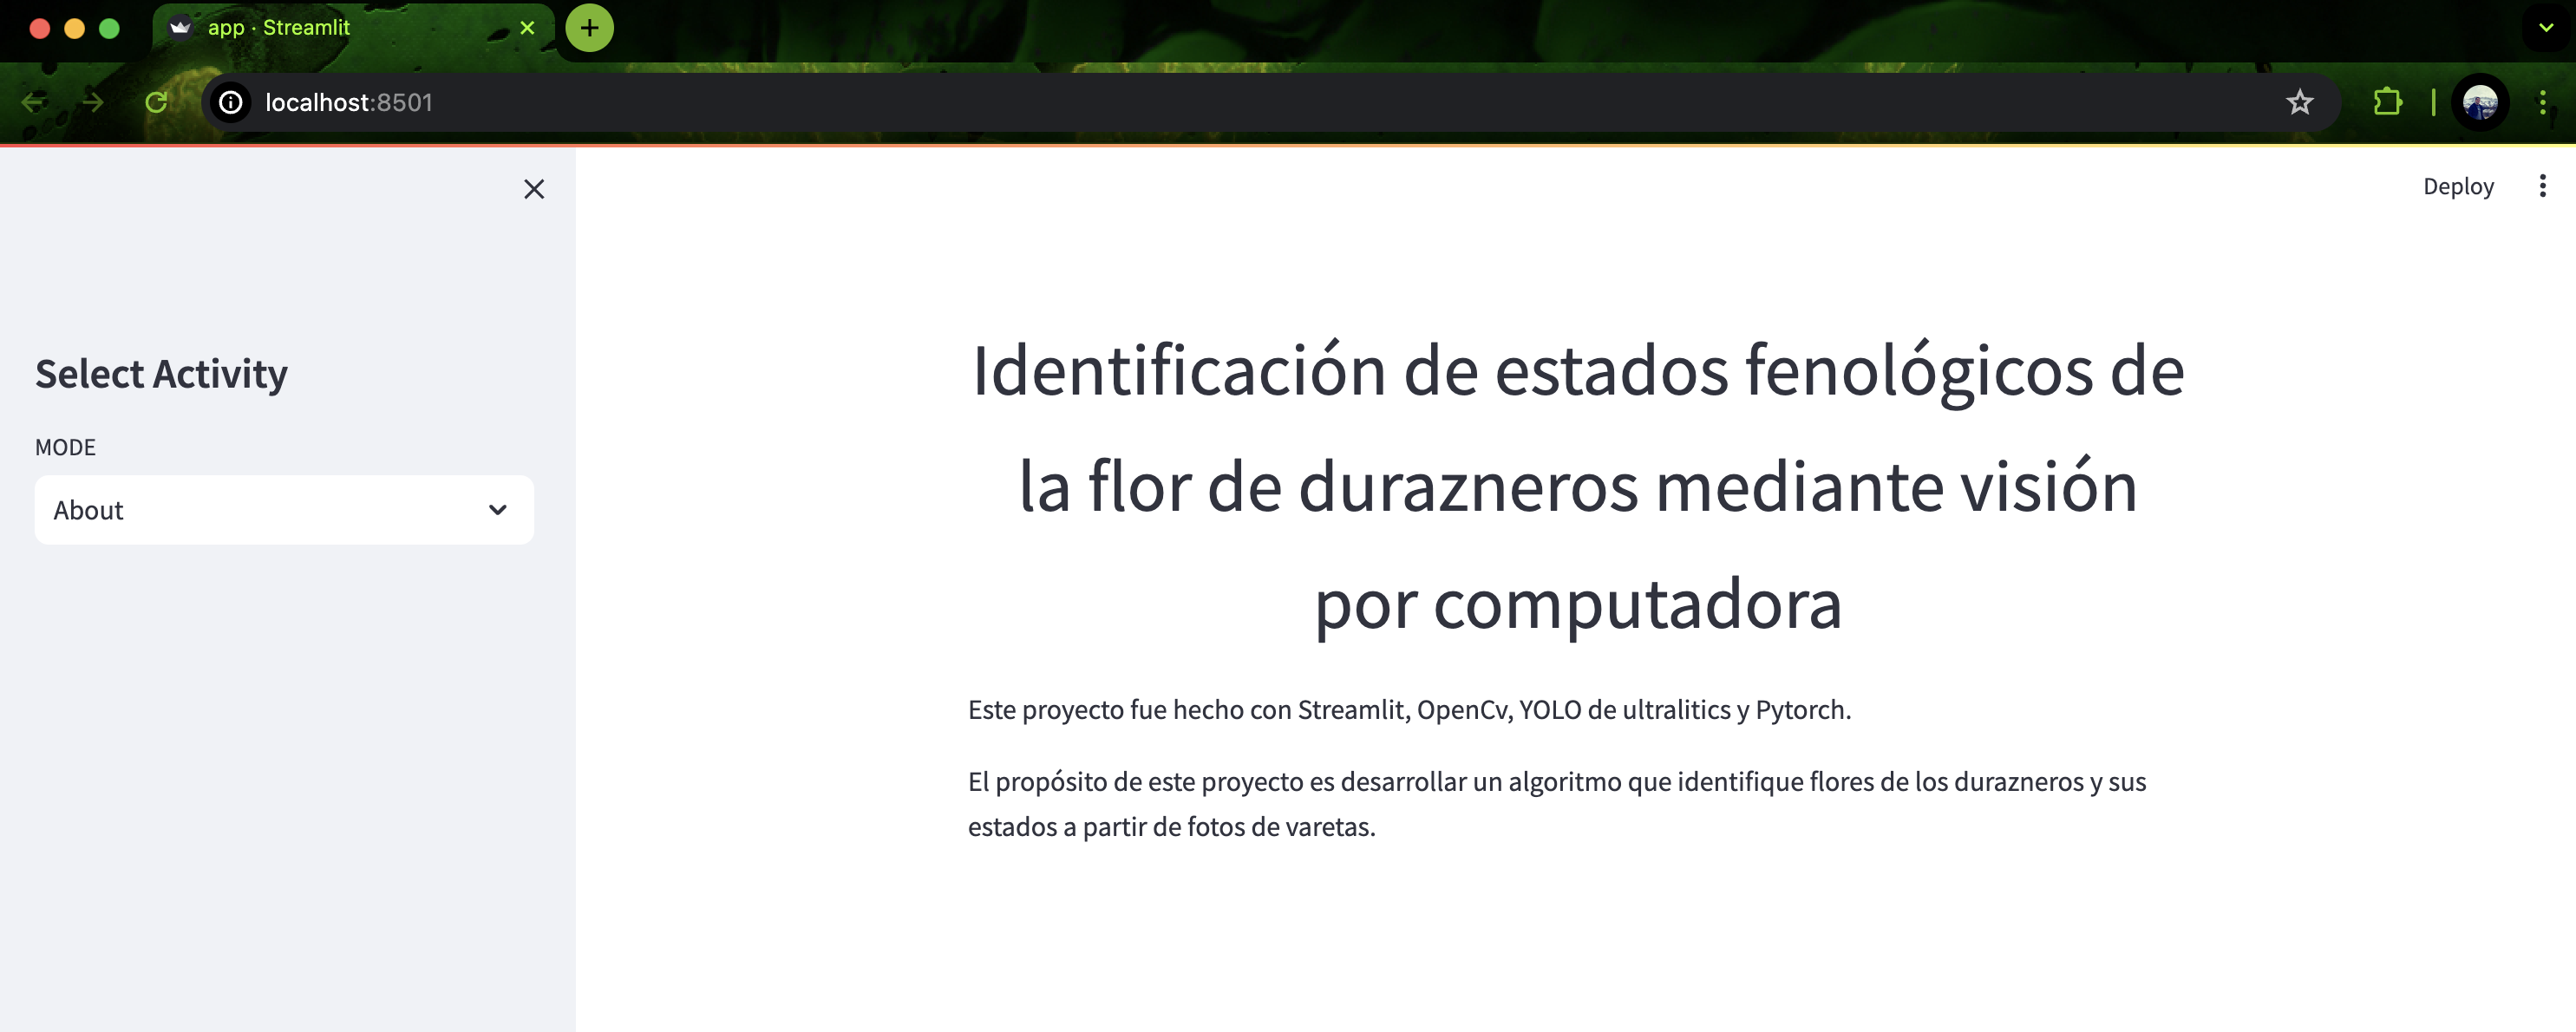
\includegraphics[scale=0.13]{./Figures/pantallaInicio.png}
	\caption{Pantalla de inicio del programa.}
	\label{fig:pantallaInicio}
\end{figure}

Como el programa se ejecuta en un entorno local, \textit{Streamlit}, utiliza el \textit{localhost} y el puerto 8501 por defecto para desplegar el sitio \textit{web}.

En el panel izquierdo se puede observar un desplegable que permite seleccionar el tipo de actividad. Para este desarrollo solo existe la detección de objetos. Al seleccionar detección de objetos, se muestra la siguiente página, donde se pedirá insertar una foto de máximo 200 MB en los formatos JPG, PNG o JPEG. La imagen se puede arrastrar directamente hasta el rectángulo de carga o se puede presionar directamente el botón de \textit{Browse files}. En la figura \ref{fig:pantalla2}, se presenta un ejemplo de esta segunda página destinada para subir la foto.

\begin{figure}[ht]
	\centering
	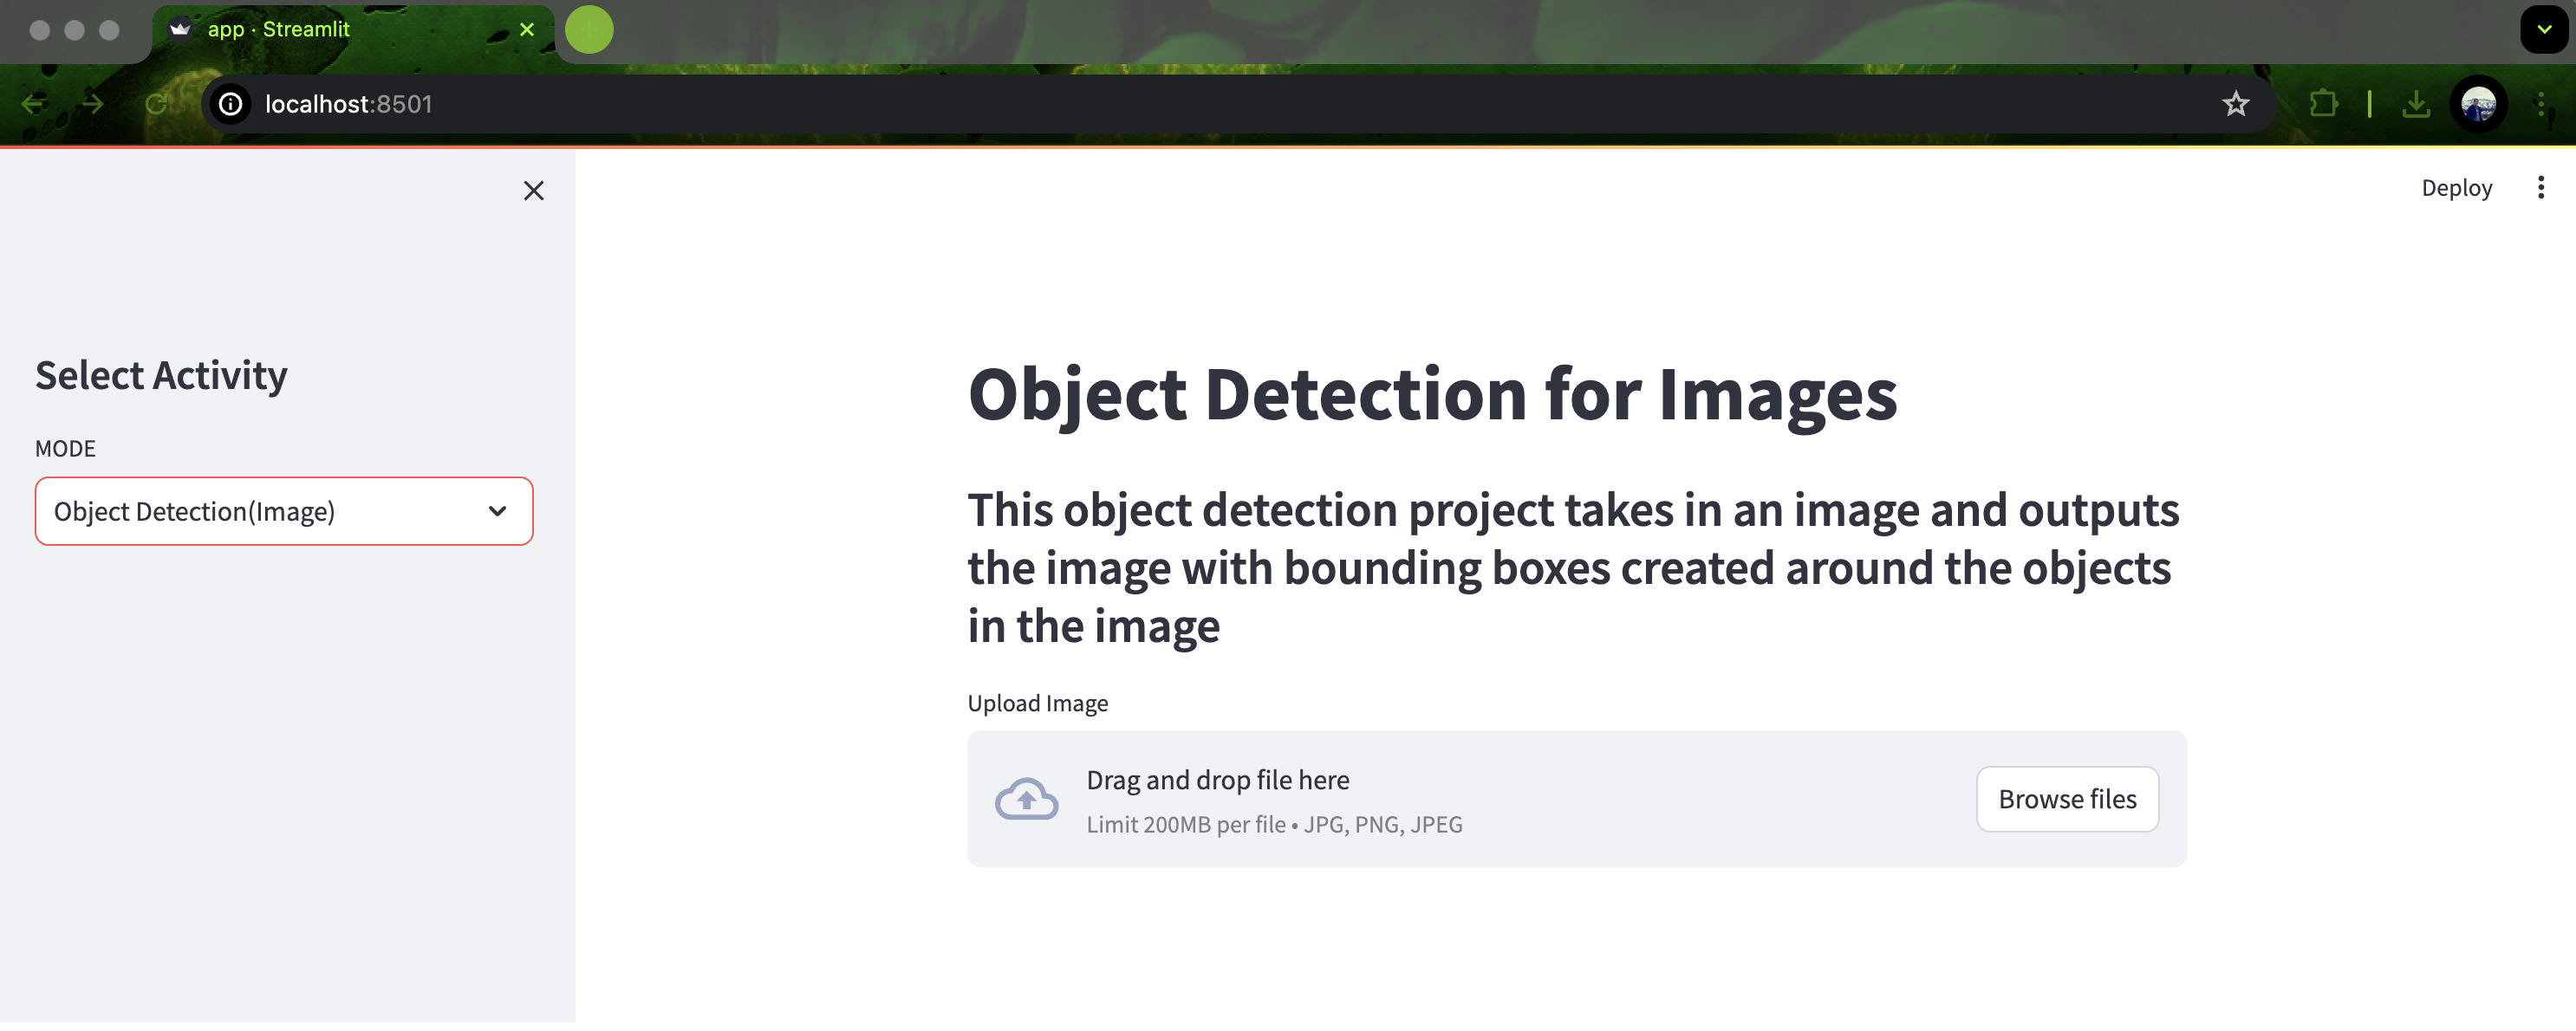
\includegraphics[scale=0.13]{./Figures/pantalla2.png}
	\caption{Página para cargar imagen.}
	\label{fig:pantalla2}
\end{figure}

Al subir una imagen, se muestra la imagen subida y se habilita una barra que modifica el parámetro de nivel de confianza (que va de un intervalo de 0 a 1) del algoritmo que detecta las varetas para el módulo de estimación de longitud y luego se habilita otra barra con el mismo propósito pero para el segundo módulo. El objetivo de estas barras es darle al INTA la flexibilidad de hacer que el algoritmo sea más estricto con las detecciones o más flexible. Por otro lado, cada barra inicia en un valor por defecto, en el caso del módulo de estimación de longitud, este valor es de 0.6 y el módulo de detección y procesamiento es de 0.4. Se seleccionaron estos valores por defecto porque son los valores donde ambos módulos en general tienen un buen rendimiento.

Las figuras \ref{fig:barra1} y \ref{fig:barra2}, se muestran dichas barras con una foto de vareta de prueba.

\begin{figure}[h]
	\centering
	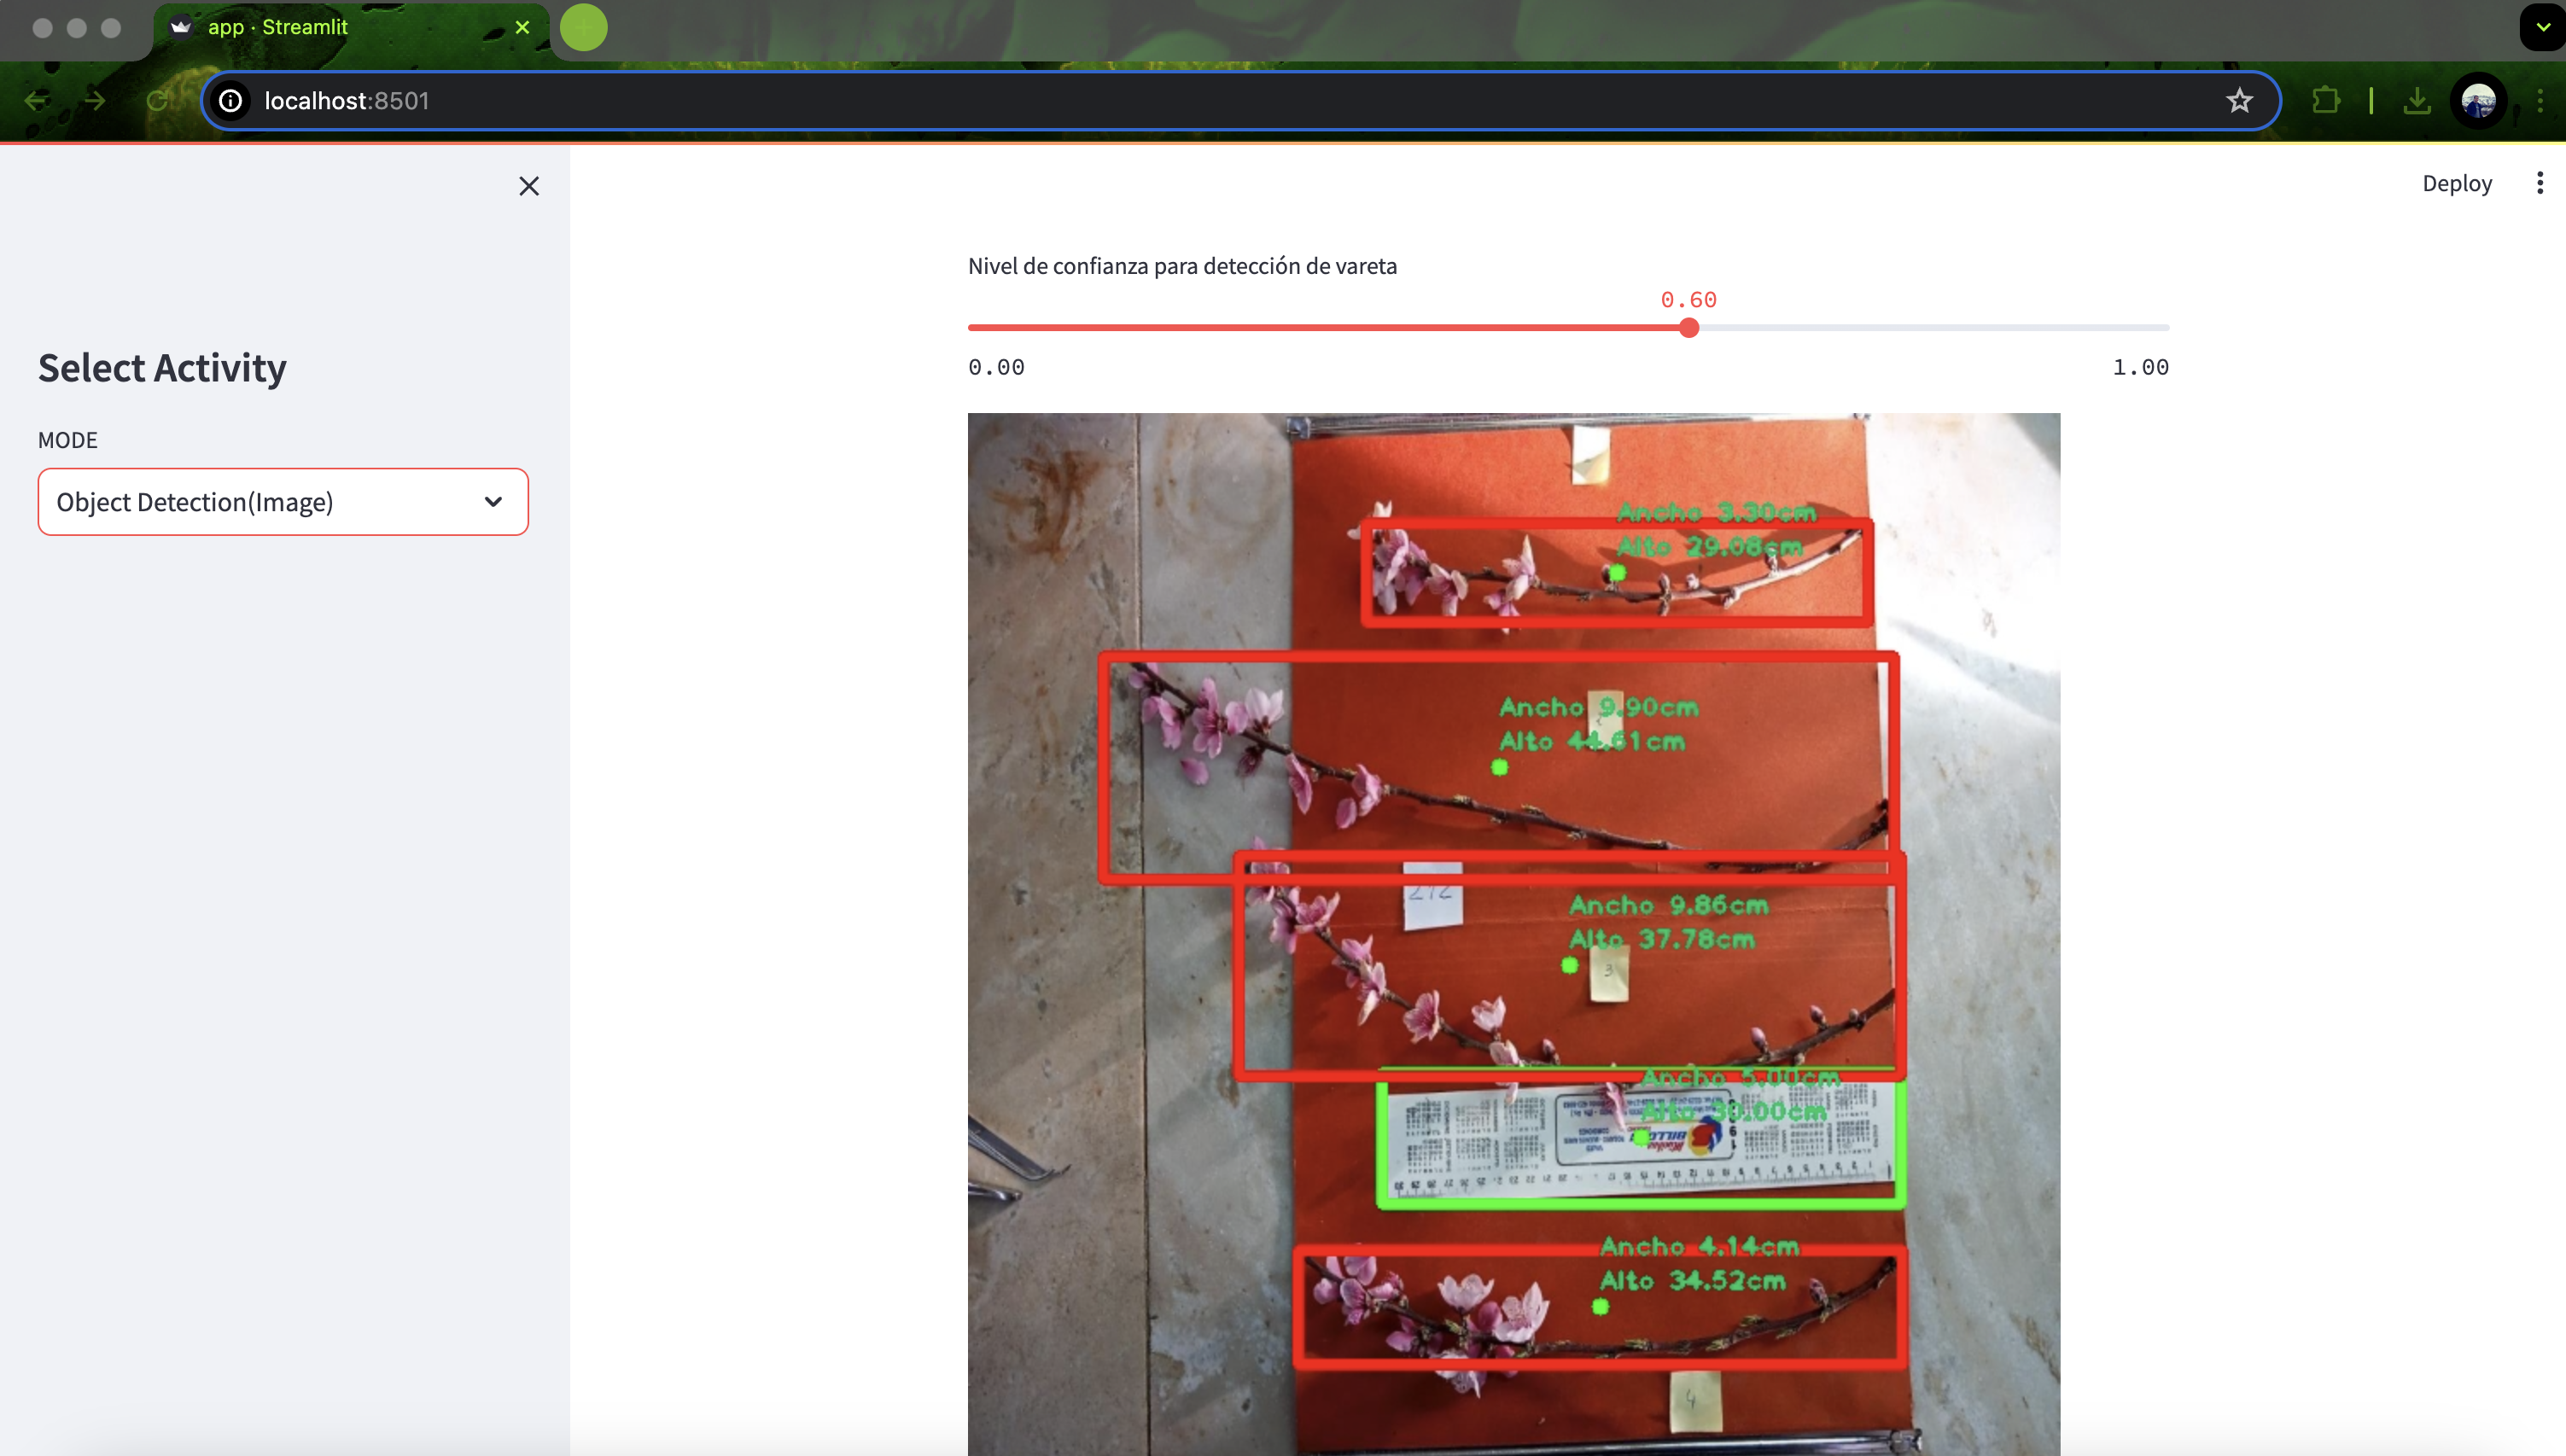
\includegraphics[scale=0.13]{./Figures/barra1.png}
	\caption{Barra de confianza para el módulo de estimación de longitud.}
	\label{fig:barra1}
\end{figure}

\newpage
\begin{figure}[ht]
	\centering
	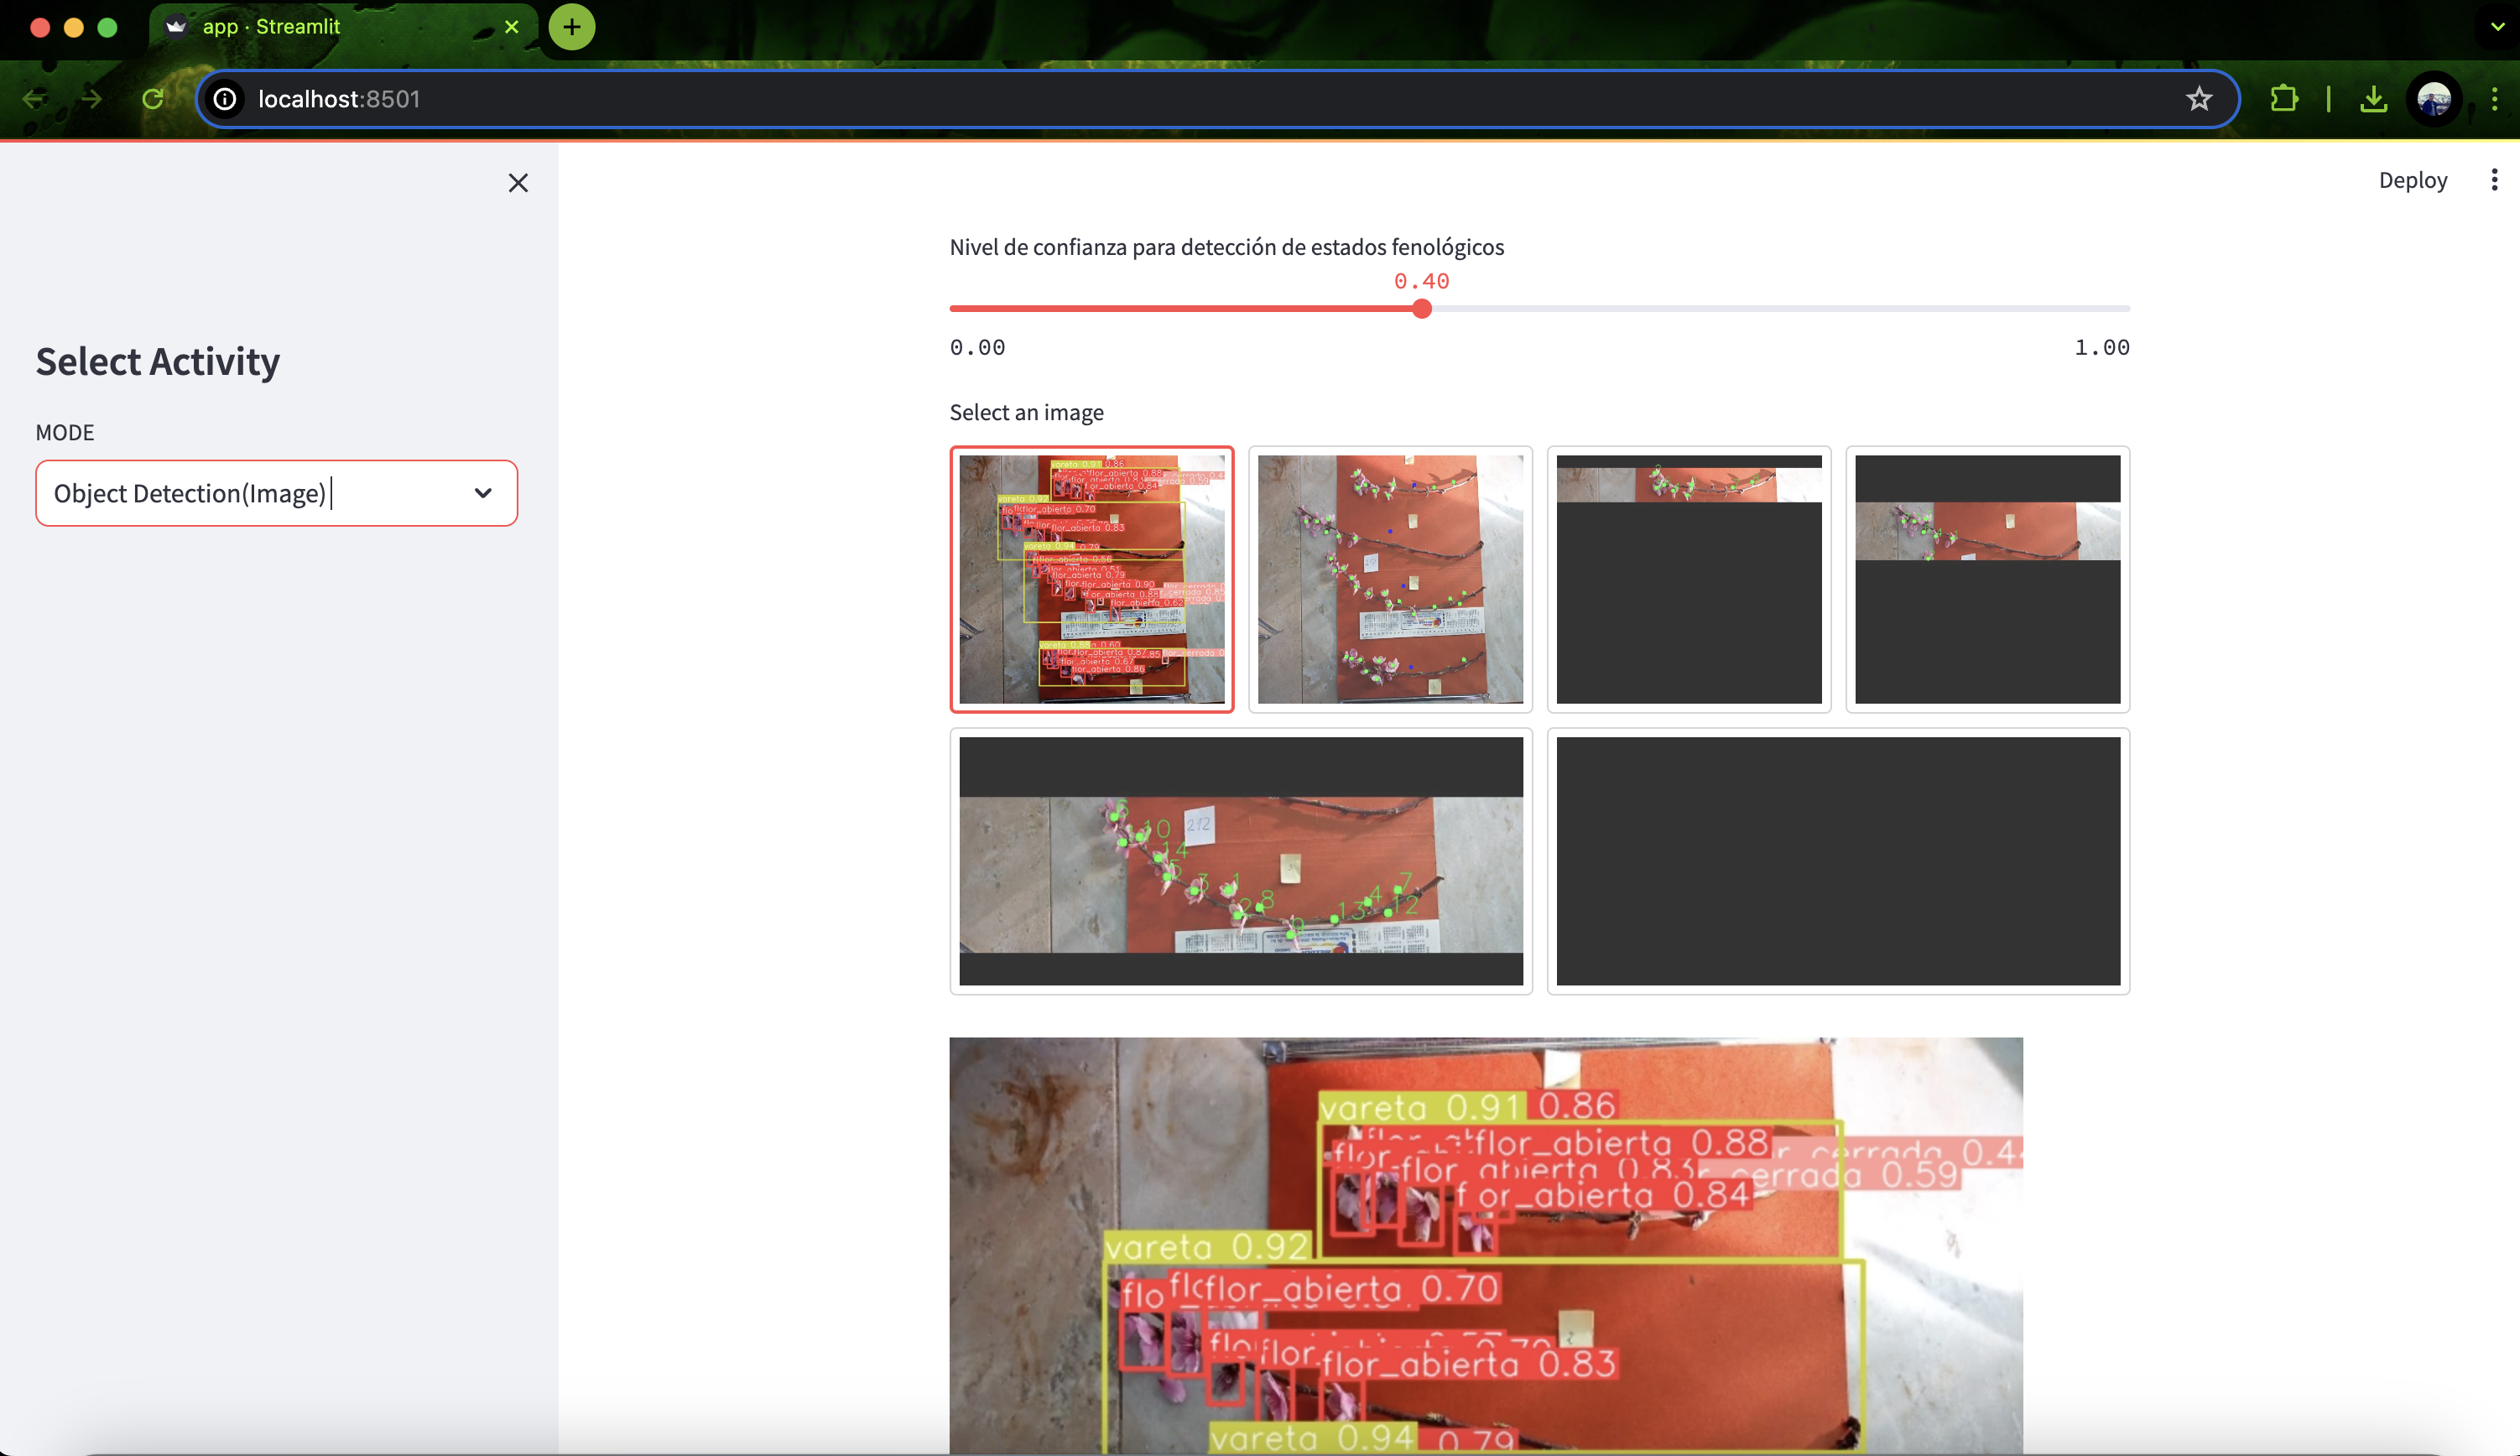
\includegraphics[scale=0.13]{./Figures/barra2.png}
	\caption{Barra de confianza para el módulo de detección y procesamiento.}
	\label{fig:barra2}
\end{figure}

Por último, al final de toda la ejecución como se mencionó anteriormente, se presentan dos botones que permiten descargar los resultados en los formatos CSV y \textit{Excel} respectivamente. En la figura \ref{fig:botonesinf}, se pueden observar dichos botones.

\begin{figure}[h]
	\centering
	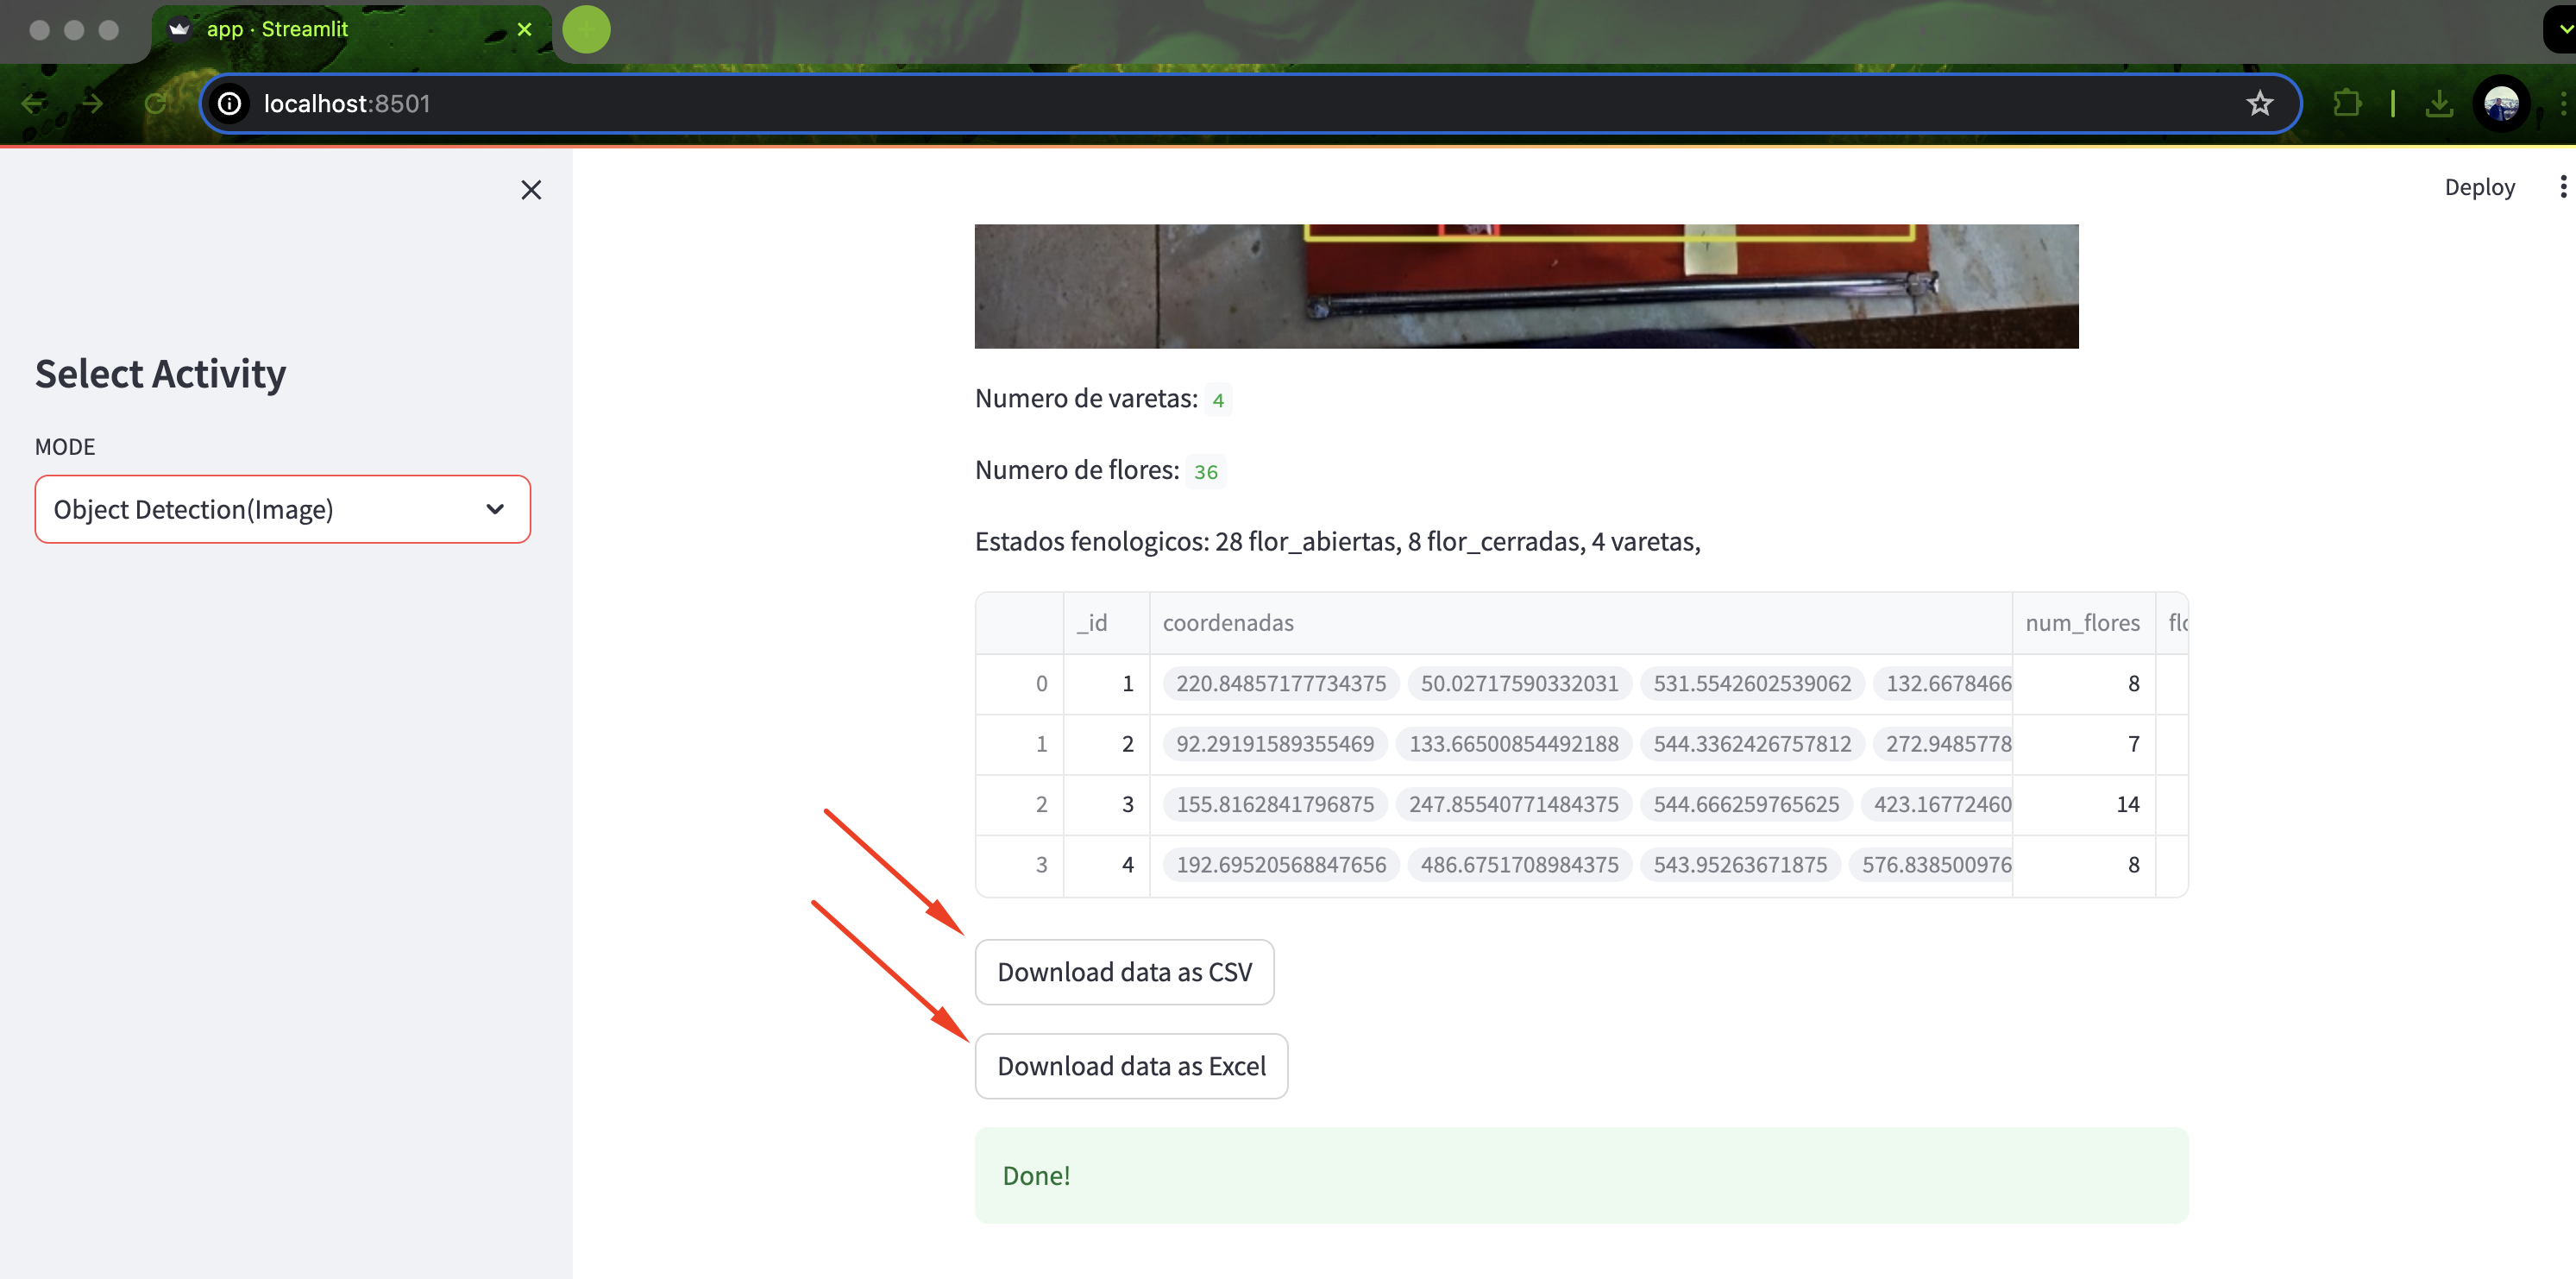
\includegraphics[scale=0.13]{./Figures/botonesinf.png}
	\caption{Botones de descarga de resultados.}
	\label{fig:botonesinf}
\end{figure}
%Este módulo como se explica en la sección \ref{section3.1}, toma como entrada una foto de vareta de duraznero y aplica un redimensionamiento, donde se reducen las dimensiones de la imagen original a una resolución de 640x640. Este primer paso es requerido, debido a que, los modelos de detección usados en esta sección, fueron preentrenados con imágenes de dichas dimensiones.
%
%El primer modelo que toma la imagen es el detector de regla. Este modelo es un YOLOv8n de Ultralytics que fue preentrenado con el conjunto de datos de COCO. Para lograr un buen rendimiento con este modelo se 




%\definecolor{mygreen}{rgb}{0,0.6,0}
%\definecolor{mygray}{rgb}{0.5,0.5,0.5}
%\definecolor{mymauve}{rgb}{0.58,0,0.82}
%
%%%%%%%%%%%%%%%%%%%%%%%%%%%%%%%%%%%%%%%%%%%%%%%%%%%%%%%%%%%%%%%%%%%%%%%%%%%%%%
%% parámetros para configurar el formato del código en los entornos lstlisting
%%%%%%%%%%%%%%%%%%%%%%%%%%%%%%%%%%%%%%%%%%%%%%%%%%%%%%%%%%%%%%%%%%%%%%%%%%%%%%
%\lstset{ %
%  backgroundcolor=\color{white},   % choose the background color; you must add \usepackage{color} or \usepackage{xcolor}
%  basicstyle=\footnotesize,        % the size of the fonts that are used for the code
%  breakatwhitespace=false,         % sets if automatic breaks should only happen at whitespace
%  breaklines=true,                 % sets automatic line breaking
%  captionpos=b,                    % sets the caption-position to bottom
%  commentstyle=\color{mygreen},    % comment style
%  deletekeywords={...},            % if you want to delete keywords from the given language
%  %escapeinside={\%*}{*)},          % if you want to add LaTeX within your code
%  %extendedchars=true,              % lets you use non-ASCII characters; for 8-bits encodings only, does not work with UTF-8
%  %frame=single,	                % adds a frame around the code
%  keepspaces=true,                 % keeps spaces in text, useful for keeping indentation of code (possibly needs columns=flexible)
%  keywordstyle=\color{blue},       % keyword style
%  language=[ANSI]C,                % the language of the code
%  %otherkeywords={*,...},           % if you want to add more keywords to the set
%  numbers=left,                    % where to put the line-numbers; possible values are (none, left, right)
%  numbersep=5pt,                   % how far the line-numbers are from the code
%  numberstyle=\tiny\color{mygray}, % the style that is used for the line-numbers
%  rulecolor=\color{black},         % if not set, the frame-color may be changed on line-breaks within not-black text (e.g. comments (green here))
%  showspaces=false,                % show spaces everywhere adding particular underscores; it overrides 'showstringspaces'
%  showstringspaces=false,          % underline spaces within strings only
%  showtabs=false,                  % show tabs within strings adding particular underscores
%  stepnumber=1,                    % the step between two line-numbers. If it's 1, each line will be numbered
%  stringstyle=\color{mymauve},     % string literal style
%  tabsize=2,	                   % sets default tabsize to 2 spaces
%  title=\lstname,                  % show the filename of files included with \lstinputlisting; also try caption instead of title
%  morecomment=[s]{/*}{*/}
%}
%
%
%%----------------------------------------------------------------------------------------
%%	SECTION 1
%%----------------------------------------------------------------------------------------
%\section{Análisis del software}
% 
%La idea de esta sección es resaltar los problemas encontrados, los criterios utilizados y la justificación de las decisiones que se hayan tomado.
%
%Se puede agregar código o pseudocódigo dentro de un entorno lstlisting con el siguiente código:
%
%\begin{verbatim}
%\begin{lstlisting}[caption= "un epígrafe descriptivo"]
%	las líneas de código irían aquí...
%\end{lstlisting}
%\end{verbatim}
%
%A modo de ejemplo:
%
%\begin{lstlisting}[label=cod:vControl,caption=Pseudocódigo del lazo principal de control.]  % Start your code-block
%
%#define MAX_SENSOR_NUMBER 3
%#define MAX_ALARM_NUMBER  6
%#define MAX_ACTUATOR_NUMBER 6
%
%uint32_t sensorValue[MAX_SENSOR_NUMBER];		
%FunctionalState alarmControl[MAX_ALARM_NUMBER];	//ENABLE or DISABLE
%state_t alarmState[MAX_ALARM_NUMBER];						//ON or OFF
%state_t actuatorState[MAX_ACTUATOR_NUMBER];			//ON or OFF
%
%void vControl() {
%
%	initGlobalVariables();
%	
%	period = 500 ms;
%		
%	while(1) {
%
%		ticks = xTaskGetTickCount();
%		
%		updateSensors();
%		
%		updateAlarms();
%		
%		controlActuators();
%		
%		vTaskDelayUntil(&ticks, period);
%	}
%}
%\end{lstlisting}



